\documentclass{article}

% Required packages (merged from hw5_template.tex and hw6_questions.tex)
\usepackage{amssymb}
\usepackage{amsmath}
\usepackage{graphicx}
\usepackage{geometry}
\usepackage{tikz}
\usepackage{array}
\usepackage{booktabs}
\usepackage{enumitem}
\usepackage{listings}
\usepackage{xcolor}
\usepackage{fancyhdr}
\usepackage{float}
\usepackage{subcaption}
\usepackage{comment}
\usepackage{algorithm}
\usepackage{algpseudocode}
\usepackage{caption}
\usepackage{siunitx}
\usepackage{hyperref}
\usetikzlibrary{arrows.meta, positioning} % Required for hw6 diagrams

% Set page geometry
\geometry{a4paper, margin=1in}

% Configure listings for Python
\lstset{
  language=Python,
  basicstyle=\ttfamily\footnotesize,
  numbers=left,
  numberstyle=\tiny\color{gray},
  frame=single,
  breaklines=true,
  breakatwhitespace=true,
  captionpos=b,
  tabsize=4,
  showspaces=false,
  showstringspaces=false,
  showtabs=false,
  commentstyle=\color{gray}\textit,
  keywordstyle=\color{blue}\bfseries,
  stringstyle=\color{red}
}

\begin{document}

\pagestyle{fancy}
\chead{DSC 257: Unsupervised Learning (Fall 2025)}
\lhead{Homework 7}
\rhead{Randall Rogers}

%------------------
% Solution for 1(a)
%------------------
\subsection*{Solution 1}
\noindent\rule{\textwidth}{0.4pt}\\
\subsubsection*{Question 1 (a)}
\begin{flushleft}
    Probability distribution $P$ over binary variables $x_1, \ldots, x_6 \in \{0, 1\}$ has the following form:
\end{flushleft}
$$
P(x_1, \ldots, x_6) = \frac{1}{Z} \psi(x_1, x_2)\psi(x_2, x_3)\psi(x_3, x_4)\psi(x_4, x_5)\psi(x_5, x_6)\psi(x_6, x_1)
$$
\begin{flushleft}
    where for $a, b \in \{0, 1\}$,
\end{flushleft}
$$
\psi(a, b) = \begin{cases}
1 & \text{if } a = b\\
0.5 & \text{otherwise}
\end{cases}
$$
\begin{flushleft}
    \textit{Draw the minimal undirected graph $G$ over which $P$ factors. (This is the undirected graph with the fewest possible edges that contains cliques corresponding to each of the terms in $P$.)}
\end{flushleft}

\subsubsection*{Solution 1 (a)}
\subsubsection*{Minimal Undirected Graph}
The given probability distribution factors into pairwise potential functions $\psi(x_i, x_j)$. According to the Hammersley-Clifford theorem, a probability distribution factors over an undirected graph $G$ if and only if it can be written as a product of potential functions over the maximal cliques of $G$. In this case, each potential function $\psi(x_i, x_{i+1})$ (with $x_7 = x_1$) corresponds to an edge between $x_i$ and $x_{i+1}$ in the graph. Since these potentials are pairwise, the graph is formed by directly connecting the variables involved in each potential.

The potential terms are:
\begin{itemize}
    \item $\psi(x_1, x_2) \implies$ edge between $x_1$ and $x_2$
    \item $\psi(x_2, x_3) \implies$ edge between $x_2$ and $x_3$
    \item $\psi(x_3, x_4) \implies$ edge between $x_3$ and $x_4$
    \item $\psi(x_4, x_5) \implies$ edge between $x_4$ and $x_5$
    \item $\psi(x_5, x_6) \implies$ edge between $x_5$ and $x_6$
    \item $\psi(x_6, x_1) \implies$ edge between $x_6$ and $x_1$
\end{itemize}
This forms a cycle graph with 6 nodes.

\begin{figure}[h!]
\centering
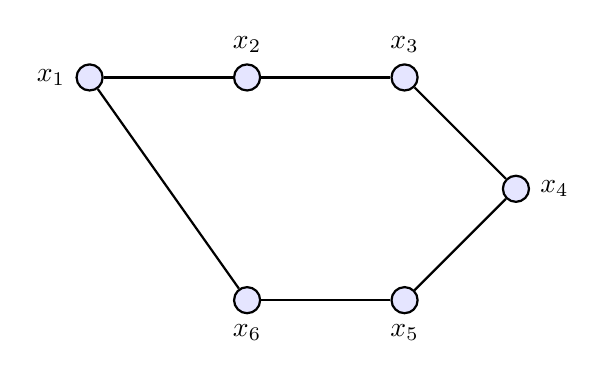
\begin{tikzpicture}[node distance=2cm, thick]
    % Nodes
    \node[circle, draw, fill=blue!10, label=left:$x_1$] (x1) {};
    \node[circle, draw, fill=blue!10, right of=x1, label=above:$x_2$] (x2) {};
    \node[circle, draw, fill=blue!10, right of=x2, label=above:$x_3$] (x3) {};
    \node[circle, draw, fill=blue!10, below right of=x3, label=right:$x_4$] (x4) {};
    \node[circle, draw, fill=blue!10, below left of=x4, label=below:$x_5$] (x5) {};
    \node[circle, draw, fill=blue!10, left of=x5, label=below:$x_6$] (x6) {};

    % Edges
    \draw (x1) -- (x2);
    \draw (x2) -- (x3);
    \draw (x3) -- (x4);
    \draw (x4) -- (x5);
    \draw (x5) -- (x6);
    \draw (x6) -- (x1);
\end{tikzpicture}
\caption{Minimal Undirected Graph for $P(x_1, \ldots, x_6)$}
\label{fig:mrf_cycle_graph}
\end{figure}

\subsubsection*{\normalfont}{$\therefore$ The minimal undirected graph is a 6-node cycle graph where each variable $x_i$ is connected to $x_{i-1}$ (or $x_6$ for $i=1$) and $x_{i+1}$ (or $x_1$ for $i=6$).}

\subsubsection*{Graduate Level Explanation}
This problem concerns the graphical representation of a pairwise Markov Random Field (MRF), specifically an Ising-like model on a cycle graph. The factorization $P(\mathbf{x}) \propto \prod_{(i,j) \in E} \psi(x_i, x_j)$ directly implies that the graph $G=(V,E)$ must have edges corresponding to each pairwise potential function. For an MRF, the set of maximal cliques in the graph dictates the factorization of the joint probability distribution. In this case, each edge $(x_i, x_{i+1})$ forms a maximal clique of size two (a pairwise clique), thus forming a cycle graph. This structure directly encodes the local dependencies defined by the potential functions.

\subsubsection*{Simple Expedited Learning Explanation}
Imagine each $x_i$ is a person, and the $\psi(x_i, x_j)$ terms are "relationships" between pairs of people. If there's a relationship between $x_1$ and $x_2$, you draw a line (an edge) connecting them. The problem lists six such relationships: $x_1$ with $x_2$, $x_2$ with $x_3$, and so on, until $x_6$ with $x_1$. When you draw all these connections, starting from $x_1$ and going around to $x_6$ and back to $x_1$, you end up with a closed loop, or a cycle graph. This graph is "minimal" because you only draw lines for the direct relationships given by the $\psi$ terms, and no extra lines.

\noindent\rule{\textwidth}{0.4pt}\\

\newpage

%------------------
% Solution for 1(b)
%------------------
\subsection*{Solution 1}
\noindent\rule{\textwidth}{0.4pt}\\
\subsubsection*{Question 1 (b)}
\begin{flushleft}
    Probability distribution $P$ over binary variables $x_1, \ldots, x_6 \in \{0, 1\}$ has the following form:
\end{flushleft}
$$
P(x_1, \ldots, x_6) = \frac{1}{Z} \psi(x_1, x_2)\psi(x_2, x_3)\psi(x_3, x_4)\psi(x_4, x_5)\psi(x_5, x_6)\psi(x_6, x_1)
$$
\begin{flushleft}
    where for $a, b \in \{0, 1\}$,
\end{flushleft}
$$
\psi(a, b) = \begin{cases}
1 & \text{if } a = b\\
0.5 & \text{otherwise}
\end{cases}
$$
\begin{flushleft}
    \textit{For what configuration(s) $x \in \{0, 1\}^6$ is $P(x)$ maximized?}
\end{flushleft}

We want to find the configuration $x = (x_1, \ldots, x_6)$ that maximizes $P(x)$.
\begin{align*}
    \arg\max_{x} P(x) &= \arg\max_{x} \left[ \frac{1}{Z} \prod_{i=1}^{5} \psi(x_i, x_{i+1}) \cdot \psi(x_6, x_1) \right]
\end{align*}
Since the partition function $Z$ is a positive constant, maximizing $P(x)$ is equivalent to maximizing the unnormalized product of potentials:
\begin{align*}
    \arg\max_{x} P(x) &= \arg\max_{x} \left[ \psi(x_1, x_2)\psi(x_2, x_3)\psi(x_3, x_4)\psi(x_4, x_5)\psi(x_5, x_6)\psi(x_6, x_1) \right]
\end{align*}
We are multiplying six potential terms together. From the definition of $\psi(a, b)$, the maximum possible value for any single potential is $\psi(a, a) = 1$. The other possible value is $\psi(a, b) = 0.5$ for $a \neq b$.

To maximize the product, we want to maximize the value of each term in the product. The largest possible product is achieved if we can make all six terms equal to 1.
This requires:
\begin{itemize}
    \item $\psi(x_1, x_2) = 1 \implies x_1 = x_2$
    \item $\psi(x_2, x_3) = 1 \implies x_2 = x_3$
    \item $\psi(x_3, x_4) = 1 \implies x_3 = x_4$
    \item $\psi(x_4, x_5) = 1 \implies x_4 = x_5$
    \item $\psi(x_5, x_6) = 1 \implies x_5 = x_6$
    \item $\psi(x_6, x_1) = 1 \implies x_6 = x_1$
\end{itemize}
Combining these conditions, we must have $x_1 = x_2 = x_3 = x_4 = x_5 = x_6$.
Since the variables are binary, $x_i \in \{0, 1\}$, there are exactly two configurations that satisfy this condition:
\begin{enumerate}
    \item $x = (0, 0, 0, 0, 0, 0)$
    \item $x = (1, 1, 1, 1, 1, 1)$
\end{enumerate}
For both of these configurations, the product of potentials is $1 \cdot 1 \cdot 1 \cdot 1 \cdot 1 \cdot 1 = 1$.
Any other configuration (e.g., $x=(0,1,0,1,0,1)$) must have at least one pair of disagreeing neighbors. For every such pair, the potential function evaluates to $0.5$. This will result in a total product strictly less than 1 (e.g., $0.5^6$ for the alternating case).
Therefore, the two configurations where all variables are aligned are the unique maximizers of $P(x)$.

\subsubsection*{\normalfont}{$\therefore$ The two configurations that maximize $P(x)$ are $x = (0, 0, 0, 0, 0, 0)$ and $x = (1, 1, 1, 1, 1, 1)$.}

\subsubsection*{Graduate Level Explanation}
This problem is a Maximum A Posteriori (MAP) inference task on a pairwise Markov Random Field. The potential function $\psi(a,b)$, which assigns a higher value to agreement ($a=b$), defines this as a **ferromagnetic Ising model**. Finding the configuration $x$ that maximizes $P(x)$ is equivalent to finding the **ground state** (minimum energy configuration) of the system. The probability $P(x) \propto \exp(-E(x))$ where $E(x) = -\sum_{(i,j)} \log \psi(x_i, x_j)$ is the energy. To maximize $P(x)$, we must minimize $E(x)$. Since $-\log(1) = 0$ and $-\log(0.5) > 0$, the energy is minimized (at $E=0$) when all neighboring "spins" are aligned. This model exhibits two degenerate ground states: all spins "down" (all 0s) and all spins "up" (all 1s).

\subsubsection*{Simple Expedited Learning Explanation}
Think of this as six friends sitting in a circle, and each must choose a "0" or a "1" hat. The "happiness" of the group is determined by multiplying "agreement scores" between all neighbors. If two neighbors have the same hat, their score $\psi$ is $1$. If they have different hats, their score is only $0.5$. To make the *total* group happiness (the final $P(x)$) as high as possible, you need every single pair of neighbors to have the highest possible score. The highest score is $1$, which happens when they match. The only way for everyone to match their neighbor in a circle is if everyone makes the same choice: either everyone wears a "0" hat, or everyone wears a "1" hat.

\noindent\rule{\textwidth}{0.4pt}\\

\newpage

%------------------
% Solution for 1(c)
%------------------
\subsection*{Solution 1}
\noindent\rule{\textwidth}{0.4pt}\\
\subsubsection*{Question 1 (c)}
\begin{flushleft}
    Probability distribution $P$ over binary variables $x_1, \ldots, x_6 \in \{0, 1\}$ has the following form:
\end{flushleft}
$$
P(x_1, \ldots, x_6) = \frac{1}{Z} \psi(x_1, x_2)\psi(x_2, x_3)\psi(x_3, x_4)\psi(x_4, x_5)\psi(x_5, x_6)\psi(x_6, x_1)
$$
\begin{flushleft}
    where for $a, b \in \{0, 1\}$,
\end{flushleft}
$$
\psi(a, b) = \begin{cases}
1 & \text{if } a = b\\
0.5 & \text{otherwise}
\end{cases}
$$
\begin{flushleft}
    \textit{For what configuration(s) $x \in \{0, 1\}^6$ is $P(x)$ minimized?}
\end{flushleft}

\subsubsection*{Solution 1 (c)}
We want to find the configuration $x = (x_1, \ldots, x_6)$ that minimizes $P(x)$.
\begin{align*}
    \arg\min_{x} P(x) &= \arg\min_{x} \left[ \frac{1}{Z} \prod_{i=1}^{5} \psi(x_i, x_{i+1}) \cdot \psi(x_6, x_1) \right]
\end{align*}
Since $Z$ is a positive constant, minimizing $P(x)$ is equivalent to minimizing the unnormalized product of potentials:
\begin{align*}
    \arg\min_{x} P(x) &= \arg\min_{x} \left[ \psi(x_1, x_2)\psi(x_2, x_3)\psi(x_3, x_4)\psi(x_4, x_5)\psi(x_5, x_6)\psi(x_6, x_1) \right]
\end{align*}
The potential function $\psi(a, b)$ has a minimum value of $0.5$, which occurs when $a \neq b$. The value is $1$ when $a = b$.

To minimize the product of these six terms, we want to make each term in the product as small as possible. The smallest possible product is achieved if we can make all six terms equal to $0.5$.
This requires that all adjacent nodes disagree:
\begin{itemize}
    \item $\psi(x_1, x_2) = 0.5 \implies x_1 \neq x_2$
    \item $\psi(x_2, x_3) = 0.5 \implies x_2 \neq x_3$
    \item $\psi(x_3, x_4) = 0.5 \implies x_3 \neq x_4$
    \item $\psi(x_4, x_5) = 0.5 \implies x_4 \neq x_5$
    \item $\psi(x_5, x_6) = 0.5 \implies x_5 \neq x_6$
    \item $\psi(x_6, x_1) = 0.5 \implies x_6 \neq x_1$
\end{itemize}
This set of conditions requires a perfectly alternating assignment of values. Let's see if this is possible.
\begin{enumerate}
    \item \textbf{Case 1: Start with $x_1 = 0$}
        \begin{itemize}
            \item $x_1 = 0 \implies x_2 = 1$
            \item $x_2 = 1 \implies x_3 = 0$
            \item $x_3 = 0 \implies x_4 = 1$
            \item $x_4 = 1 \implies x_5 = 0$
            \item $x_5 = 0 \implies x_6 = 1$
            \item \textbf{Check final link:} We need $x_6 \neq x_1$. Here, $x_6 = 1$ and $x_1 = 0$. This condition is satisfied.
            \item This gives the configuration: $x = (0, 1, 0, 1, 0, 1)$.
        \end{itemize}
    \item \textbf{Case 2: Start with $x_1 = 1$}
        \begin{itemize}
            \item $x_1 = 1 \implies x_2 = 0$
            \item $x_2 = 0 \implies x_3 = 1$
            \item $x_3 = 1 \implies x_4 = 0$
            \item $x_4 = 0 \implies x_5 = 1$
            \item $x_5 = 1 \implies x_6 = 0$
            \item \textbf{Check final link:} We need $x_6 \neq x_1$. Here, $x_6 = 0$ and $x_1 = 1$. This condition is satisfied.
            \item This gives the configuration: $x = (1, 0, 1, 0, 1, 0)$.
        \end{itemize}
\end{enumerate}
These two alternating configurations both result in a product of potentials equal to $0.5^6 = 0.015625$. Any other configuration must have at least one pair of agreeing neighbors, e.g., $\psi(x_i, x_{i+1}) = 1$. This would make the product $1 \cdot 0.5^5 = 0.03125$ (or larger), which is greater than $0.5^6$.
Therefore, the two alternating configurations are the unique minimizers.

\subsubsection*{\normalfont}{$\therefore$ The two configurations that minimize $P(x)$ are the alternating patterns: $x = (0, 1, 0, 1, 0, 1)$ and $x = (1, 0, 1, 0, 1, 0)$.}

\subsubsection*{Graduate Level Explanation}
This problem asks for the maximum energy (minimum probability) states of a ferromagnetic Ising model. The potential $\psi(a,b)$ penalizes disagreement, so the highest energy states are those with the most disagreements. The underlying graph is a 6-cycle, which is a **bipartite graph** (a graph whose vertices can be divided into two disjoint sets such that every edge connects a vertex in one set to one in the other). For a bipartite graph, a 2-coloring is possible, which corresponds exactly to an assignment where no two adjacent nodes have the same value. The two configurations found, $(0,1,0,1,0,1)$ and $(1,0,1,0,1,0)$, represent the two valid 2-colorings of this graph. These states maximize the system's energy (minimize probability) by maximizing the number of "unhappy" (disagreeing) links. This is only possible without **frustration** because the cycle length is even.

\subsubsection*{Simple Expedited Learning Explanation}
Following the "six friends in a circle" analogy, we now want to find the configuration that makes the group *unhappiest*. The group's "happiness score" is $1$ if neighbors match and only $0.5$ if they differ. To get the lowest possible total score (the minimum $P(x)$), we need every single pair of neighbors to get the lowest score of $0.5$. This means everyone must have a different hat from their neighbors. If person 1 picks "0", person 2 must pick "1", person 3 must pick "0", and so on. This creates an alternating pattern $(0, 1, 0, 1, 0, 1)$. We check the last link: person 6 (with "1") is different from person 1 (with "0"), so it works! The only other possibility is starting with "1", which gives the other alternating pattern $(1, 0, 1, 0, 1, 0)$.

\noindent\rule{\textwidth}{0.4pt}\\

\newpage

%------------------
% Solution for 2(a)
%------------------
\subsection*{Solution 2}
\noindent\rule{\textwidth}{0.4pt}\\
\subsubsection*{Question 2 (a)}
\begin{flushleft}
In a tournament, each player plays three games. Define three random variables:
\begin{itemize}
\item Random variable $A$ is 1 if Tom wins his first game, and is 0 otherwise.
\item Random variable $B$ is 1 if Tom wins his first two games, and is 0 otherwise.
\item Random variable $C$ is 1 if Tom wins all three of his games, and is 0 otherwise.
\end{itemize}
\textit{Is $C$ independent of $A$ (i.e., is it true that for any values $a, c$ that $A, C$ might take on, we have $\Pr(A = a, C = c) = \Pr(A = a)\Pr(C = c)$)? Give a brief (one-sentence) reason for your answer.} 
\end{flushleft}
\begin{flushleft}
    \textit{Hint: The answer is no; show this by exhibiting specific choices of $a, c$ for which $\Pr(A = a, C = c) \neq \Pr(A = a)\Pr(C = c)$.}
\end{flushleft}

\subsubsection*{Solution 2 (a)}
We follow the hint and test the case where $a=0$ and $c=1$.
\begin{itemize}
    \item $A=0$ is the event "Tom does not win his first game."
    \item $C=1$ is the event "Tom wins all three of his games."
\end{itemize}
By definition, the event $C=1$ implies that Tom wins Game 1, Game 2, and Game 3. This means that $C=1$ and $A=0$ are mutually exclusive events; it is impossible for Tom to lose his first game *and* win all three games.

Therefore, the joint probability is $\Pr(A=0, C=1) = 0$.

Now we consider the product of the marginal probabilities, $\Pr(A=0)\Pr(C=1)$.
Let's assume the probability of winning any game $i$ is $p_i$, where $0 < p_i < 1$. This means the games are non-deterministic (it's possible to both win and lose).
\begin{itemize}
    \item $\Pr(A=0) = \Pr(\text{Lose Game 1}) = 1 - p_1$. Since $p_1 < 1$, we have $\Pr(A=0) > 0$.
    \item $\Pr(C=1) = \Pr(\text{Win G1, G2, G3})$. Assuming game independence, $\Pr(C=1) = p_1 p_2 p_3$. Since $p_i > 0$, we have $\Pr(C=1) > 0$.
\end{itemize}
The product of the marginals is $\Pr(A=0)\Pr(C=1) = (1 - p_1)(p_1 p_2 p_3)$, which is strictly greater than 0.

We have found a case where $\Pr(A=0, C=1) = 0$ but $\Pr(A=0)\Pr(C=1) > 0$.
Since $0 \neq (1-p_1)(p_1 p_2 p_3)$, the independence condition $\Pr(A=a, C=c) = \Pr(A=a)\Pr(C=c)$ is violated.

\subsubsection*{\normalfont}{$\therefore$ No, $C$ is not independent of $A$ because if Tom loses his first game ($A=0$), he *cannot* win all three games ($C=1$), so $\Pr(A=0, C=1)=0$, which is not equal to the product $\Pr(A=0)\Pr(C=1)$ (as both marginal probabilities are non-zero, assuming non-trivial games).}

\subsubsection*{Graduate Level Explanation}
The variables $A$ and $C$ are not marginally independent because a deterministic, causal relationship exists between them. Specifically, $C$ is a logical subset of $A$; the event $C=1$ (winning all three) *implies* the event $A=1$ (winning the first). Therefore, $\Pr(C=1 \mid A=0) = 0$. For independence to hold, this conditional probability must equal the marginal probability $\Pr(C=1)$, but $\Pr(C=1) > 0$ (assuming a non-zero chance of winning). Because $\Pr(C=1 \mid A=0) \neq \Pr(C=1)$, they are dependent; observing $A=0$ provides definitive information about $C$ (namely, that $C=0$).

\subsubsection*{Simple Expedited Learning Explanation}
No. Think of it this way: "Winning all three games" ($C=1$) *includes* "Winning the first game" ($A=1$). They are not separate events. If I tell you "Tom lost the first game" ($A=0$), you know *for sure* that "Tom won all three games" ($C=1$) is false. Since knowing the outcome of $A$ gives you 100\% certainty about $C$ in this case, they are clearly dependent.

\newpage

%------------------
% Solution for 2(b)
%------------------
\subsection*{Solution 2}
\noindent\rule{\textwidth}{0.4pt}\\
\subsubsection*{Question 2 (b)}
\begin{flushleft}
In a tournament, each player plays three games. Define three random variables:
\begin{itemize}
\item Random variable $A$ is 1 if Tom wins his first game, and is 0 otherwise.
\item Random variable $B$ is 1 if Tom wins his first two games, and is 0 otherwise.
\item Random variable $C$ is 1 if Tom wins all three of his games, and is 0 otherwise.
\end{itemize}
\textit{Is $C$ conditionally independent of $A$ given $B$ (i.e., is it true that $\Pr(C = c|A = a, B = b) = \Pr(C = c|B = b)$)? Give a brief reason.} 
\end{flushleft}

\subsubsection*{Solution 2 (b)}
Yes, $C$ is conditionally independent of $A$ given $B$. We can prove this by checking all possible values of the conditioning variable $B$.

Let $p_3 = \Pr(\text{Win Game 3} \mid \text{Win Game 1, Win Game 2})$. We assume $0 < p_3 < 1$.

\begin{enumerate}
    \item \textbf{Case 1: We condition on $B=1$ (Tom wins the first two games).}
        \begin{itemize}
            \item If $B=1$, then $A$ *must* be 1 (winning the first two games implies winning the first game). The case $A=0, B=1$ has zero probability, so we only need to check $A=1, B=1$.
            \item $\Pr(C=1 \mid B=1)$: Given Tom won the first two games, the probability of winning all three is just the probability of winning Game 3. So, $\Pr(C=1 \mid B=1) = p_3$.
            \item $\Pr(C=1 \mid A=1, B=1)$: Given Tom won the first game ($A=1$) AND won the first two games ($B=1$), the $A=1$ information is redundant. The probability of winning all three is still just the probability of winning Game 3. So, $\Pr(C=1 \mid A=1, B=1) = p_3$.
            \item In this case, $\Pr(C \mid A, B=1) = \Pr(C \mid B=1)$.
        \end{itemize}
    \item \textbf{Case 2: We condition on $B=0$ (Tom does not win the first two games).}
        \begin{itemize}
            \item If Tom did not win the first two games, it is impossible for him to win all three games.
            \item $\Pr(C=1 \mid B=0) = 0$.
            \item Now we check $\Pr(C=1 \mid A, B=0)$ for both values of $A$:
                \item $\Pr(C=1 \mid A=0, B=0)$: Given Tom lost the first game ($A=0$), it is impossible to win all three. This probability is 0.
                \item $\Pr(C=1 \mid A=1, B=0)$: Given Tom won the first game ($A=1$) but failed to win the first two ($B=0$) (i.e., he lost Game 2), it is impossible to win all three. This probability is 0.
            \item In all sub-cases where $B=0$, $\Pr(C=1 \mid A, B=0) = 0$, which equals $\Pr(C=1 \mid B=0)$.
        \end{itemize}
\end{enumerate}
Since $\Pr(C \mid A, B) = \Pr(C \mid B)$ holds for all possible values of $A, B, C$, the conditional independence statement is true.

\subsubsection*{\normalfont}{$\therefore$ Yes, $C$ is conditionally independent of $A$ given $B$, because once we know the outcome of the first two games ($B$), knowing the outcome of *only* the first game ($A$) provides no new information for predicting the outcome of all three games ($C$).}

\subsubsection*{Graduate Level Explanation}
Yes. The probabilistic relationships $A \leftarrow B \leftarrow C$ form a **Markov chain** (where $C=1 \implies B=1 \implies A=1$). A fundamental property of Markov chains is that, given the "present" state ($B$), the "future" ($C$) is conditionally independent of the "past" ($A$). The variable $B$ acts as an information bottleneck; it "screens off" any influence $A$ has on $C$. Any path from $A$ to $C$ in the dependency graph must pass through $B$, so conditioning on $B$ blocks this path, satisfying the definition of d-separation.

\subsubsection*{Simple Expedited Learning Explanation}
Yes. Think of $B$ as a "gate". To predict $C$ (winning all 3 games), you only need to know two things:
\begin{enumerate}
    \item Did Tom pass the gate $B$ (win the first two games)?
    \item Did Tom win Game 3?
\end{enumerate}
If I tell you $B=0$ (he didn't pass the gate), you know $C$ is 0 (he can't win all 3). It doesn't matter *why* he failed $B$ (whether he lost G1 or G2).
If I tell you $B=1$ (he passed the gate), all you care about now is Game 3. Does it help to *also* tell you $A=1$ (he won Game 1)? No, you already knew that, because $B=1$ *means* he won Game 1 and Game 2.
Since $B$ tells you everything $A$ could, and more, $B$ makes $A$ redundant.

\noindent\rule{\textwidth}{0.4pt}\\

\newpage

%------------------
% Solution for 2(c)
%------------------
\subsection*{Solution 2}
\noindent\rule{\textwidth}{0.4pt}\\
\subsubsection*{Question 2 (c)}
\begin{flushleft}
In a tournament, each player plays three games. Define three random variables:
\begin{itemize}
\item Random variable $A$ is 1 if Tom wins his first game, and is 0 otherwise.
\item Random variable $B$ is 1 if Tom wins his first two games, and is 0 otherwise.
\item Random variable $C$ is 1 if Tom wins all three of his games, and is 0 otherwise.
\end{itemize}
\textit{Draw an undirected graphical model for $(A, B, C)$.} 
\end{flushleft}

\subsubsection*{Solution 2 (c)}
\subsubsection*{Solution 2 (c)}
\subsubsection*{Undirected Graphical Model}
An undirected graphical model (UGM) represents conditional independencies. An edge is absent between two nodes $X$ and $Y$ if they are conditionally independent given all other variables in the graph.

From our answer in 2(b), we proved the key conditional independence relationship: $A \perp C \mid B$.
This means that in our undirected graph, the node $B$ must separate nodes $A$ and $C$. The only way to achieve this in a three-node graph is to *not* have a direct edge between $A$ and $C$.

We must also check if other edges are required:
\begin{itemize}
    \item \textbf{Edge (A, B):} Are $A$ and $B$ conditionally independent given $C$? No. For example, if $C=0$, knowing $A=0$ makes $B=0$ certain, while knowing $A=1$ does not ( $B$ could be 0 or 1, though $B=1$ is impossible if $C=0$). Since $A \not\perp B \mid C$, we need an edge between $A$ and $B$.
    \item \textbf{Edge (B, C):} Are $B$ and $C$ conditionally independent given $A$? No. If $A=1$, knowing $B=0$ (lost G2) makes $C=0$ certain, while knowing $B=1$ (won G1 \& G2) makes $C$ uncertain (depends on G3). Since $B \not\perp C \mid A$, we need an edge between $B$ and $C$.
\end{itemize}
The graph must therefore have edges $(A, B)$ and $(B, C)$, but no edge $(A, C)$. This forms a simple chain.

\begin{figure}[h!]
\centering
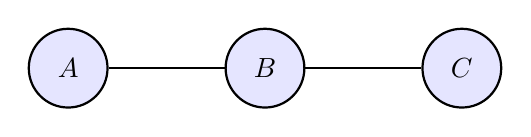
\begin{tikzpicture}[node distance=2.5cm, thick, scale=1.0, every node/.style={transform shape}]
    \node[circle, draw, fill=blue!10, minimum size=1cm] (A) {$A$};
    \node[circle, draw, fill=blue!10, minimum size=1cm, right of=A] (B) {$B$};
    \node[circle, draw, fill=blue!10, minimum size=1cm, right of=B] (C) {$C$};
    
    \draw (A) -- (B);
    \draw (B) -- (C);
\end{tikzpicture}
\caption{Undirected Graphical Model for $(A, B, C)$}
\label{fig:ugm_abc}
\end{figure}

\subsubsection*{\normalfont}{$\therefore$ The undirected graphical model is the chain $A - B - C$, which correctly encodes the relationship that $A$ and $C$ are conditionally independent given $B$.}

\subsubsection*{Graduate Level Explanation}
The minimal directed acyclic graph (DAG) that captures the dependency structure is the Markov chain $A \to B \to C$. This is because the event $B$ (winning G1 \& G2) depends on $A$ (winning G1), and $C$ (winning G1, G2, \& G3) depends on $B$. This DAG encodes the conditional independence $A \perp C \mid B$ via d-separation. To find the minimal undirected graph (the "moral graph") that preserves this independence, we apply the moralization procedure: 1) "Marry" (connect) all pairs of non-adjacent parents, and 2) Drop all arrowheads. Since there are no nodes with multiple parents (no v-structures), no edges are added. Dropping the arrows from $A \to B \to C$ directly yields the UGM $A - B - C$.

\subsubsection*{Simple Expedited Learning Explanation}
Think of the graph as showing who "talks to" whom.
\begin{itemize}
    \item $A$ (Win G1) talks directly to $B$ (Win G1 \& G2), because $B$'s outcome is built from $A$'s.
    \item $C$ (Win G1, G2, \& G3) talks directly to $B$ (Win G1 \& G2), because $C$'s outcome is built from $B$'s.
    \item $A$ and $C$ do *not* talk directly. $C$ gets all the information it needs about $A$ *through* $B$.
\end{itemize}
Therefore, we draw a line from $A$ to $B$, and from $B$ to $C$. The resulting picture is just a simple chain: $A - B - C$. The missing line between $A$ and $C$ is the most important part: it means "if you know $B$, $A$ and $C$ have nothing left to say to each other."

\noindent\rule{\textwidth}{0.4pt}\\

\newpage

%------------------
% Solution for 3 (a)
%------------------
\subsection*{Solution 3}
\noindent\rule{\textwidth}{0.4pt}\\
\subsubsection*{Question 3 (a)}
\begin{flushleft}
    Four random variables $W, X, Y, Z$ factor over the graph shown below.
\end{flushleft}
\begin{center}
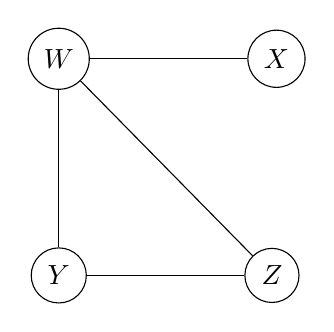
\begin{tikzpicture}[node distance=2cm]
\node[circle,draw] (W) {$W$};
\node[circle,draw,right=of W] (X) {$X$};
\node[circle,draw,below=of W] (Y) {$Y$};
\node[circle,draw,right=of Y] (Z) {$Z$};
\draw (W) -- (X);
\draw (Y) -- (W);
\draw (Y) -- (Z);
\draw (W) -- (Z);
\end{tikzpicture}
\end{center}

\begin{flushleft}
    \textit{What is the functional form of the joint distribution $P(W, X, Y, Z)$?}
\end{flushleft}

\subsubsection*{Solution 3 (a)}
\subsubsection*{Solution 3 (a)}
According to the **Hammersley-Clifford theorem**, any positive probability distribution $P$ that factors over an undirected graph $G$ can be written as a product of potential functions ($\psi_C$) over the **maximal cliques** of the graph, normalized by a partition function $Z$.

\begin{enumerate}
    \item \textbf{Define a Clique:} A clique is a subset of nodes in the graph where every node in the subset is connected to every other node in the subset.
    \item \textbf{Define a Maximal Clique:} A clique is *maximal* if it is not a subset of any larger clique.
    \item \textbf{Identify Cliques in G:}
        \begin{itemize}
            \item \textit{Size 2 (edges):} $\{W, X\}$, $\{W, Y\}$, $\{W, Z\}$, $\{Y, Z\}$
            \item \textit{Size 3 (triangles):} We check subsets of size 3.
                \begin{itemize}
                    \item $\{W, Y, Z\}$: The edges are $(W,Y)$, $(W,Z)$, and $(Y,Z)$. All three edges exist. This is a clique.
                    \item $\{W, X, Y\}$: The edges are $(W,X)$, $(W,Y)$, and $(X,Y)$. The edge $(X,Y)$ is missing. This is not a clique.
                    \item $\{W, X, Z\}$: The edges are $(W,X)$, $(W,Z)$, and $(X,Z)$. The edge $(X,Z)$ is missing. This is not a clique.
                \end{itemize}
            \item \textit{Size 4:} $\{W, X, Y, Z\}$ is not a clique (e.g., $(X,Y)$ is missing).
        \end{itemize}
    \item \textbf{Identify Maximal Cliques $\mathcal{C}$:}
        \begin{itemize}
            \item Is $\{W, Y, Z\}$ maximal? Yes. It is a clique, and we cannot add the only remaining node $X$ (as $X$ is not connected to $Y$ or $Z$).
            \item Is $\{W, X\}$ maximal? Yes. It is a clique, and we cannot add $Y$ (no $X-Y$ edge) or $Z$ (no $X-Z$ edge).
            \item The other cliques, $\{W, Y\}$, $\{W, Z\}$, and $\{Y, Z\}$, are *not* maximal because they are all subsets of the larger clique $\{W, Y, Z\}$.
        \end{itemize}
    \item \textbf{Construct Functional Form:} The set of maximal cliques is $\mathcal{C} = \{\{W, X\}, \{W, Y, Z\}\}$. The joint distribution is the product of potentials over these two cliques.
\end{enumerate}


\subsubsection*{\normalfont}{$\therefore$ The functional form is $P(W, X, Y, Z) = \frac{1}{Z} \psi_1(W, X) \psi_2(W, Y, Z)$, where $Z$ is the partition function, defined as $Z = \sum_{w,x,y,z} \psi_1(w, x) \psi_2(w, y, z)$.}

\subsubsection*{Graduate Level Explanation}
The Hammersley-Clifford theorem establishes the equivalence between the conditional independence properties of an undirected graphical model (a Markov Random Field) and its factorization into a product of potentials over its maximal cliques. This form of distribution is also known as a **Gibbs distribution**. The graph's topology, $G=(V,E)$, defines the set of maximal cliques $\mathcal{C}$. Here, $\mathcal{C} = \{\{W, X\}, \{W, Y, Z\}\}$. This factorization implies all the conditional independencies in the graph, such as $X \perp \{Y, Z\} \mid W$, which can be verified by graph separation.

\subsubsection*{Simple Expedited Learning Explanation}
Think of the graph as a network of "friend groups" where everyone in a group is friends with everyone else. These groups are "cliques." We are looking for the *biggest* friend groups that can't add any new members (these are "maximal cliques").
\begin{itemize}
    \item $W, Y, Z$ are all friends with each other, forming a trio. They can't add $X$ because $X$ isn't friends with $Y$ or $Z$. So, $\{W, Y, Z\}$ is one maximal group.
    \item $W, X$ are friends. They can't add $Y$ (not friends with $X$) or $Z$ (not friends with $X$). So, $\{W, X\}$ is another maximal group.
\end{itemize}
The total probability of the system is just the "score" of the $\{W, X\}$ group multiplied by the "score" of the $\{W, Y, Z\}$ group, all divided by a number $Z$ to make sure the probabilities add up to 1.

\noindent\rule{\textwidth}{0.4pt}\\

\newpage

%------------------
% Solution for 3 (b)
%------------------
\subsection*{Solution 3}
\noindent\rule{\textwidth}{0.4pt}\\
\subsubsection*{Question 3 (b)}
\begin{flushleft}
    Four random variables $W, X, Y, Z$ factor over the graph shown below.
\end{flushleft}
\begin{center}
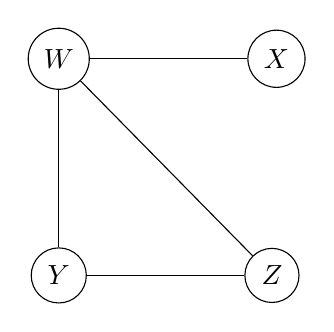
\begin{tikzpicture}[node distance=2cm]
\node[circle,draw] (W) {$W$};
\node[circle,draw,right=of W] (X) {$X$};
\node[circle,draw,below=of W] (Y) {$Y$};
\node[circle,draw,right=of Y] (Z) {$Z$};
\draw (W) -- (X);
\draw (Y) -- (W);
\draw (Y) -- (Z);
\draw (W) -- (Z);
\end{tikzpicture}
\end{center}

\begin{flushleft}
    \textit{Write down a conditional independence property of this distribution.}
\end{flushleft}

\subsubsection*{Solution 3 (b)}
In an undirected graphical model, conditional independence is determined by **graph separation**. A set of nodes $A$ is conditionally independent of a set of nodes $B$ given a set of nodes $C$ (written $A \perp B \mid C$) if $C$ separates $A$ and $B$. This means that every path from any node in $A$ to any node in $B$ must pass through at least one node in $C$.

Let's test the independence between $X$ and the set $\{Y, Z\}$.
\begin{itemize}
    \item Let $A = \{X\}$.
    \item Let $B = \{Y, Z\}$.
    \item Let's test if $C = \{W\}$ is a separating set.
\end{itemize}
We must check all paths from $A$ to $B$:
\begin{enumerate}
    \item \textbf{Paths from $X$ to $Y$:} The two paths are $X-W-Y$ and $X-W-Z-Y$. Both of these paths pass through $W$.
    \item \textbf{Paths from $X$ to $Z$:} The two paths are $X-W-Z$ and $X-W-Y-Z$. Both of these paths also pass through $W$.
\end{enumerate}
Since every possible path from $X$ to any node in $\{Y, Z\}$ is blocked by (i.e., must pass through) the node $W$, the set $C=\{W\}$ separates $A=\{X\}$ from $B=\{Y, Z\}$.

Therefore, the distribution must satisfy the conditional independence property $X \perp \{Y, Z\} \mid W$.

\subsubsection*{\normalfont}{$\therefore$ A conditional independence property of this distribution is $X \perp \{Y, Z\} \mid W$ (or $X \perp Y \mid W$, or $X \perp Z \mid W$, which are also true).}

\subsubsection*{Graduate Level Explanation}
The graph $G$ implies a set of conditional independencies defined by the **Global Markov Property**: for any disjoint sets $A, B, C$, if $C$ separates $A$ from $B$, then $A \perp B \mid C$. The node $W$ acts as an **articulation point** (or separating set) between node $X$ and the subgraph induced by $\{Y, Z\}$. The factorization found in 3(a), $P \propto \psi_1(W,X)\psi_2(W,Y,Z)$, also implies this. When we condition on $W$, the joint distribution $P(X, Y, Z \mid W)$ becomes proportional to $\psi_1(W, X) \psi_2(W, Y, Z)$. Since $X$ only appears in the first potential and $\{Y, Z\}$ only in the second, the distribution factors as $P(X \mid W) P(Y, Z \mid W)$, which is the definition of $X \perp \{Y, Z\} \mid W$.

\subsubsection*{Simple Expedited Learning Explanation}
Think of the graph lines as information channels. $X$ can only send or receive information to $Y$ or $Z$ by going *through* $W$. The node $W$ is the "gatekeeper" for $X$. If we "condition on $W$", it means we are standing at the gate $W$ and we already know its value. Once we know $W$'s value, $X$ has no *new* information to tell $Y$ or $Z$, and $Y$ and $Z$ have no *new* information to tell $X$. By observing the gatekeeper $W$, we "block" the channel of influence, making $X$ and the pair $\{Y, Z\}$ independent of each other.
\newpage


%------------------
% Solution for 4(a)
%------------------
\subsection*{Solution 4}
\noindent\rule{\textwidth}{0.4pt}\\
\subsubsection*{Question 4 (a)}
\begin{flushleft}
    The joint distribution $P$ over $(x_1, x_2, x_3)$ is given by the following table.
\end{flushleft}
\begin{center}
\begin{tabular}{c|c|c|c}
$x_1$ & $x_2$ & $x_3$ & Pr \\\hline
0 & 0 & 0 & 1/3 \\
0 & 0 & 1 & 1/3 \\
1 & 0 & 0 & 1/6 \\
1 & 1 & 1 & 1/6
\end{tabular}
\end{center}

\begin{flushleft}
    \textit{One of these variables is a deterministic function of the other two. Identify this relationship.}
\end{flushleft}

\subsubsection*{Solution 4 (a)}
A variable $Y$ is a deterministic function of $X$ and $Z$ if, for every pair of values $(x, z)$ that has a non-zero probability of occurring, there is only one possible value for $y$. We inspect the four configurations in the table that have non-zero probability.

\begin{enumerate}
    \item \textbf{Is $x_1 = f(x_2, x_3)$?}
    No. We test the input $(x_2=0, x_3=0)$.
    \begin{itemize}
        \item Row 1: $(x_2=0, x_3=0)$ maps to $x_1=0$.
        \item Row 3: $(x_2=0, x_3=0)$ maps to $x_1=1$.
    \end{itemize}
    Since a single input maps to multiple outputs, $x_1$ is not a deterministic function of $x_2$ and $x_3$.

    \item \textbf{Is $x_3 = f(x_1, x_2)$?}
    No. We test the input $(x_1=0, x_2=0)$.
    \begin{itemize}
        \item Row 1: $(x_1=0, x_2=0)$ maps to $x_3=0$.
        \item Row 2: $(x_1=0, x_2=0)$ maps to $x_3=1$.
    \end{itemize}
    Since a single input maps to multiple outputs, $x_3$ is not a deterministic function of $x_1$ and $x_2$.

    \item \textbf{Is $x_2 = f(x_1, x_3)$?}
    Yes. We test all input pairs $(x_1, x_3)$ that appear in the table:
    \begin{itemize}
        \item Row 1: Input $(x_1=0, x_3=0)$ maps to $x_2=0$.
        \item Row 2: Input $(x_1=0, x_3=1)$ maps to $x_2=0$.
        \item Row 3: Input $(x_1=1, x_3=0)$ maps to $x_2=0$.
        \item Row 4: Input $(x_1=1, x_3=1)$ maps to $x_2=1$.
    \end{itemize}
    In every case, a given input pair $(x_1, x_3)$ maps to a single, unique output for $x_2$. We can summarize this function in a truth table:
    \begin{center}
    \begin{tabular}{cc|c}
    $x_1$ & $x_3$ & $x_2$ \\\hline
    0 & 0 & 0 \\
    0 & 1 & 0 \\
    1 & 0 & 0 \\
    1 & 1 & 1
    \end{tabular}
    \end{center}
    This is the truth table for the logical AND operation.
\end{enumerate}

\subsubsection*{\normalfont}{$\therefore$ The deterministic relationship is $x_2 = x_1 \land x_3$ (i.e., $x_2$ is 1 if and only if $x_1=1$ and $x_3=1$).}

\subsubsection*{Graduate Level Explanation}
The support of the joint distribution $P(x_1, x_2, x_3)$ (the set of configurations with non-zero probability) is a strict subset of the full space $\{0, 1\}^3$. This implies that at least one conditional probability is deterministic (has zero entropy). By inspection, we find that the conditional distribution $P(x_2 \mid x_1, x_3)$ is deterministic for all $(x_1, x_3)$ in the support of the marginal $P(x_1, x_3)$. Specifically, $P(x_2 \mid x_1, x_3) = \delta(x_2, x_1 \land x_3)$, where $\delta$ is the Kronecker delta. This functional dependence means the joint distribution can be factored as $P(x_1, x_2, x_3) = P(x_1, x_3) P(x_2 \mid x_1, x_3)$.

\subsubsection*{Simple Expedited Learning Explanation}
Look at the four rows in the table that are "allowed" (have non-zero probability). We are looking for a rule where two columns perfectly predict the third.
\begin{itemize}
    \item Try to predict $x_2$ using $x_1$ and $x_3$.
    \item Row 1: $x_1=0, x_3=0$. The $x_2$ is $0$.
    \item Row 2: $x_1=0, x_3=1$. The $x_2$ is $0$.
    \item Row 3: $x_1=1, x_3=0$. The $x_2$ is $0$.
    \item Row 4: $x_1=1, x_3=1$. The $x_2$ is $1$.
\end{itemize}
This rule works every time. Notice that $x_2$ is $1$ *only when* $x_1$ AND $x_3$ are both $1$. In all other cases, $x_2$ is $0$. This is the logical "AND" rule.

\newpage

%------------------
% Solution for 4(b)
%------------------
\subsection*{Solution 4}
\noindent\rule{\textwidth}{0.4pt}\\
\subsubsection*{Question 4 (b)}
\begin{flushleft}
    The joint distribution $P$ over $(x_1, x_2, x_3)$ is given by the following table.
\end{flushleft}
\begin{center}
\begin{tabular}{c|c|c|c}
$x_1$ & $x_2$ & $x_3$ & Pr \\\hline
0 & 0 & 0 & 1/3 \\
0 & 0 & 1 & 1/3 \\
1 & 0 & 0 & 1/6 \\
1 & 1 & 1 & 1/6
\end{tabular}
\end{center}

\begin{flushleft}
    \textit{Draw the minimal Bayes net $G$ over which this distribution factors.}
\end{flushleft}
\begin{flushleft}
    \textit{Hint: Start from (a), which shows that one variable is fully determined by the other two; are the latter two variables independent or not?}
\end{flushleft}

\subsubsection*{Solution 4 (b)}
A Bayes net $G$ provides a factorization of the joint distribution $P(x_1, x_2, x_3) = \prod_i P(x_i \mid \text{parents}_G(x_i))$.
From 4(a), we know $x_2$ is a deterministic function of $x_1$ and $x_3$, namely $x_2 = x_1 \land x_3$. This means $P(x_2 \mid x_1, x_3)$ is deterministic (1 for $x_2 = x_1 \land x_3$ and 0 otherwise). This strongly suggests a structure where $x_1$ and $x_3$ are parents of $x_2$, i.e., $x_1 \to x_2 \leftarrow x_3$.

This v-structure implies the factorization $P(x_1, x_2, x_3) = P(x_1)P(x_3)P(x_2 \mid x_1, x_3)$. This factorization is valid if and only if $x_1$ and $x_3$ are marginally independent ($x_1 \perp x_3$).

We must test this independence by computing the marginals from the table:
\begin{itemize}
    \item \textbf{Marginal $P(x_1)$:}
        \begin{itemize}
            \item $\Pr(x_1=0) = \Pr(0,0,0) + \Pr(0,0,1) = 1/3 + 1/3 = 2/3$
            \item $\Pr(x_1=1) = \Pr(1,0,0) + \Pr(1,1,1) = 1/6 + 1/6 = 1/3$
        \end{itemize}
    \item \textbf{Marginal $P(x_3)$:}
        \begin{itemize}
            \item $\Pr(x_3=0) = \Pr(0,0,0) + \Pr(1,0,0) = 1/3 + 1/6 = 3/6 = 1/2$
            \item $\Pr(x_3=1) = \Pr(0,0,1) + \Pr(1,1,1) = 1/3 + 1/6 = 3/6 = 1/2$
        \end{itemize}
    \item \textbf{Joint $P(x_1, x_3)$:} (Summing over $x_2$)
        \begin{itemize}
            \item $\Pr(x_1=0, x_3=0) = \Pr(0,0,0) = 1/3$
            \item $\Pr(x_1=0, x_3=1) = \Pr(0,0,1) = 1/3$
            \item $\Pr(x_1=1, x_3=0) = \Pr(1,0,0) = 1/6$
            \item $\Pr(x_1=1, x_3=1) = \Pr(1,1,1) = 1/6$
        \end{itemize}
\end{itemize}
\textbf{Check for independence:} $\Pr(x_1, x_3) \stackrel{?}{=} \Pr(x_1)\Pr(x_3)$
\begin{itemize}
    \item $\Pr(x_1=0)\Pr(x_3=0) = (2/3)(1/2) = 1/3$. This equals $\Pr(x_1=0, x_3=0)$.
    \item $\Pr(x_1=0)\Pr(x_3=1) = (2/3)(1/2) = 1/3$. This equals $\Pr(x_1=0, x_3=1)$.
    \item $\Pr(x_1=1)\Pr(x_3=0) = (1/3)(1/2) = 1/6$. This equals $\Pr(x_1=1, x_3=0)$.
    \item $\Pr(x_1=1)\Pr(x_3=1) = (1/3)(1/2) = 1/6$. This equals $\Pr(x_1=1, x_3=1)$.
\end{itemize}
Since $P(x_1, x_3) = P(x_1)P(x_3)$ holds for all combinations, $x_1$ and $x_3$ are indeed marginally independent.
The minimal Bayes net is therefore the one that encodes $x_1 \perp x_3$ and the dependency $x_2 = f(x_1, x_3)$. This is the v-structure $x_1 \to x_2 \leftarrow x_3$.

\begin{figure}[h!]
\centering
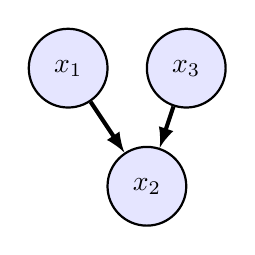
\begin{tikzpicture}[node distance=1.5cm and 2cm, thick]
    \node[circle, draw, fill=blue!10, minimum size=1cm] (x1) {$x_1$};
    \node[circle, draw, fill=blue!10, minimum size=1cm, right of=x1] (x3) {$x_3$};
    \node[circle, draw, fill=blue!10, minimum size=1cm, below of=x1, xshift=1cm] (x2) {$x_2$};
    
    \draw[->, >=latex, line width=1.5pt] (x1) -- (x2);
    \draw[->, >=latex, line width=1.5pt] (x3) -- (x2);
\end{tikzpicture}
\caption{Minimal Bayes Net for $P(x_1, x_2, x_3)$}
\label{fig:v_structure}
\end{figure}

\subsubsection*{\normalfont}{$\therefore$ The minimal Bayes net is the v-structure $x_1 \to x_2 \leftarrow x_3$, as $x_1$ and $x_3$ are marginally independent, and $x_2$ is a deterministic function of both.}

\subsubsection*{Graduate Level Explanation}
The distribution's support reveals a deterministic conditional $P(x_2 \mid x_1, x_3) = \delta(x_2, x_1 \land x_3)$. This necessitates $x_1$ and $x_3$ being parents of $x_2$. The marginal independence $x_1 \perp x_3$, which we verified via calculation, implies there are no edges or other paths between $x_1$ and $x_3$. The resulting graph, $x_1 \to x_2 \leftarrow x_3$, is a **v-structure**, also known as a **collider**. This minimal directed acyclic graph (DAG) correctly encodes the marginal independence of the parents ($x_1 \perp x_3$) while also encoding a conditional dependence ($x_1 \not\perp x_3 \mid x_2$) via the "explaining away" phenomenon.

\subsubsection*{Simple Expedited Learning Explanation}
In 4(a) we found that $x_2$ is built using $x_1$ and $x_3$ (specifically, an "AND" rule). In a Bayes net, this means $x_1$ and $x_3$ are the "parents," and we draw arrows from them *to* $x_2$: $x_1 \to x_2 \leftarrow x_3$. The only other question is whether $x_1$ and $x_3$ are connected. We checked the probabilities and found that $x_1$ and $x_3$ are completely independent, like two separate coin flips. Since they are independent, we do not draw any edge between them. The final, minimal graph is just the two parents pointing to their child.

\noindent\rule{\textwidth}{0.4pt}\\

\newpage

%------------------
% Solution for 4(c)
%------------------
\subsection*{Solution 4}
\noindent\rule{\textwidth}{0.4pt}\\
\subsubsection*{Question 4 (c)}
\begin{flushleft}
    The joint distribution $P$ over $(x_1, x_2, x_3)$ is given by the following table.
\end{flushleft}
\begin{center}
\begin{tabular}{c|c|c|c}
$x_1$ & $x_2$ & $x_3$ & Pr \\\hline
0 & 0 & 0 & 1/3 \\
0 & 0 & 1 & 1/3 \\
1 & 0 & 0 & 1/6 \\
1 & 1 & 1 & 1/6
\end{tabular}
\end{center}

\begin{flushleft}
    \textit{Now show how $P$ factors over $G$ by explicitly giving the three (conditional) probability tables, one per $x_i$.}
\end{flushleft}

\subsubsection*{Solution 4 (c)}
From 4(b), we know the minimal Bayes net is the v-structure $x_1 \to x_2 \leftarrow x_3$. The joint distribution thus factors as $P(x_1, x_2, x_3) = P(x_1) P(x_3) P(x_2 \mid x_1, x_3)$.
We need to find the three (Conditional) Probability Tables (CPTs) for $P(x_1)$, $P(x_3)$, and $P(x_2 \mid x_1, x_3)$.

\textbf{1. CPT for $x_1$:}
We find the marginal probability $P(x_1)$ by summing over $x_2$ and $x_3$ in the joint table.
\begin{itemize}
    \item $\Pr(x_1=0) = \Pr(0,0,0) + \Pr(0,0,1) = 1/3 + 1/3 = 2/3$
    \item $\Pr(x_1=1) = \Pr(1,0,0) + \Pr(1,1,1) = 1/6 + 1/6 = 2/6 = 1/3$
\end{itemize}
\begin{center}
\begin{tabular}{c|c}
$x_1$ & $\Pr(x_1)$ \\\hline
0 & 2/3 \\
1 & 1/3
\end{tabular}
\end{center}

\textbf{2. CPT for $x_3$:}
We find the marginal probability $P(x_3)$ by summing over $x_1$ and $x_2$.
\begin{itemize}
    \item $\Pr(x_3=0) = \Pr(0,0,0) + \Pr(1,0,0) = 1/3 + 1/6 = 2/6 + 1/6 = 1/2$
    \item $\Pr(x_3=1) = \Pr(0,0,1) + \Pr(1,1,1) = 1/3 + 1/6 = 2/6 + 1/6 = 1/2$
\end{itemize}
\begin{center}
\begin{tabular}{c|c}
$x_3$ & $\Pr(x_3)$ \\\hline
0 & 1/2 \\
1 & 1/2
\end{tabular}
\end{center}

\textbf{3. CPT for $x_2$:}
We need the conditional probability $P(x_2 \mid x_1, x_3)$. From 4(a), we know this is a deterministic relationship: $x_2 = x_1 \land x_3$. This means $\Pr(x_2=1 \mid x_1, x_3)$ is 1 if and only if $x_1=1$ and $x_3=1$. For all other parent combinations, $\Pr(x_2=0 \mid x_1, x_3) = 1$.
\begin{center}
\begin{tabular}{cc|c|c}
$x_1$ & $x_3$ & $\Pr(x_2=0 \mid x_1, x_3)$ & $\Pr(x_2=1 \mid x_1, x_3)$ \\\hline
0 & 0 & 1 & 0 \\
0 & 1 & 1 & 0 \\
1 & 0 & 1 & 0 \\
1 & 1 & 0 & 1
\end{tabular}
\end{center}
\textit{Verification:} We can check one row of the original table. $\Pr(x_1=0, x_2=0, x_3=1) = P(x_1=0)P(x_3=1)P(x_2=0 \mid x_1=0, x_3=1) = (2/3) \cdot (1/2) \cdot (1) = 2/6 = 1/3$. This matches the original table.

\subsubsection*{\normalfont}{$\therefore$ The three tables are $P(x_1)$ (with $\Pr(x_1=1)=1/3$), $P(x_3)$ (with $\Pr(x_3=1)=1/2$), and the deterministic CPT for $P(x_2 \mid x_1, x_3)$ which implements the $x_2 = x_1 \land x_3$ function.}

\subsubsection*{Graduate Level Explanation}
The chain rule for Bayes nets asserts that $P(\mathbf{X}) = \prod_{i} P(X_i \mid \text{Pa}_G(X_i))$. For our minimal DAG $G$ where $\text{Pa}(x_1)=\emptyset$, $\text{Pa}(x_3)=\emptyset$, and $\text{Pa}(x_2)=\{x_1, x_3\}$, this becomes $P(x_1, x_2, x_3) = P(x_1)P(x_3)P(x_2 \mid x_1, x_3)$. The CPTs for the root nodes $x_1$ and $x_3$ are their marginal distributions, which we found by summing out the other variables. The CPT for the child $x_2$ is **degenerate** (contains only 0s and 1s), reflecting the deterministic functional relationship in the joint distribution's support.

\subsubsection*{Simple Expedited Learning Explanation}
The Bayes net $x_1 \to x_2 \leftarrow x_3$ is a "recipe" for building the full probability table. These CPTs are the "ingredients."
\begin{enumerate}
    \item \textbf{Table 1 ($P(x_1)$):} "Flip a biased coin for $x_1$. It lands on '1' 1/3 of the time."
    \item \textbf{Table 2 ($P(x_3)$):} "Flip a fair coin for $x_3$. It lands on '1' 1/2 of the time."
    \item \textbf{Table 3 ($P(x_2 \mid \ldots)$):} "Look at the results of $x_1$ and $x_3$. Set $x_2$ to 1 *if and only if* both $x_1$ and $x_3$ were 1. Otherwise, set $x_2$ to 0."
\end{enumerate}
These three simple tables store all the information from the original (and more complex) joint table.

\noindent\rule{\textwidth}{0.4pt}\\

\newpage

%------------------
% Solution for 4(d)
%------------------
\subsection*{Solution 4}
\noindent\rule{\textwidth}{0.4pt}\\
\subsubsection*{Question 4 (d)}
\begin{flushleft}
    The joint distribution $P$ over $(x_1, x_2, x_3)$ is given by the following table.
\end{flushleft}
\begin{center}
\begin{tabular}{c|c|c|c}
$x_1$ & $x_2$ & $x_3$ & Pr \\\hline
0 & 0 & 0 & 1/3 \\
0 & 0 & 1 & 1/3 \\
1 & 0 & 0 & 1/6 \\
1 & 1 & 1 & 1/6
\end{tabular}
\end{center}

\begin{flushleft}
    \textit{Draw the minimal undirected graph $G'$ over which distribution $P$ factors.}
\end{flushleft}

\subsubsection*{Solution 4 (d)}
The minimal undirected graph $G'$ that represents a distribution $P$ can be derived from its minimal Bayes net $G$ (found in 4(b)) using the process of **moralization**.

\begin{enumerate}
    \item \textbf{Start with the Bayes Net $G$:} From 4(b), the minimal DAG was the v-structure $x_1 \to x_2 \leftarrow x_3$.
    \item \textbf{"Marry the parents":} Add an undirected edge between all pairs of nodes that have a common child. In $G$, $x_1$ and $x_3$ are both parents of $x_2$. Since they are not already connected, we must add the "moral" edge $x_1 - x_3$.
    \item \textbf{Drop all arrowheads:} Convert all directed edges to undirected edges. This turns $x_1 \to x_2$ into $x_1 - x_2$ and $x_3 \to x_2$ into $x_3 - x_2$.
\end{enumerate}

The resulting graph $G'$ has three edges: $(x_1, x_2)$, $(x_2, x_3)$, and the new moral edge $(x_1, x_3)$. This forms a fully connected graph, or a 3-clique.

\begin{figure}[h!]
\centering
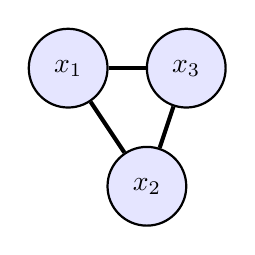
\begin{tikzpicture}[node distance=1.5cm and 2cm, thick, scale=1.0, every node/.style={transform shape}]
    \node[circle, draw, fill=blue!10, minimum size=1cm] (x1) {$x_1$};
    \node[circle, draw, fill=blue!10, minimum size=1cm, right of=x1] (x3) {$x_3$};
    \node[circle, draw, fill=blue!10, minimum size=1cm, below of=x1, xshift=1cm] (x2) {$x_2$};
    
    \draw[line width=1.5pt] (x1) -- (x2);
    \draw[line width=1.5pt] (x3) -- (x2);
    % The "moral" edge
    \draw[line width=1.5pt] (x1) -- (x3);
\end{tikzpicture}
\caption{Minimal Undirected Graph $G'$}
\label{fig:ugm_moralized}
\end{figure}

This graph is minimal because the distribution $P$ contains no conditional independence properties. For example, $x_1$ and $x_3$ are *not* independent given $x_2$ (this is "explaining away"). Any UGM with fewer edges (e.g., $x_1 - x_2 - x_3$) would incorrectly imply $x_1 \perp x_3 \mid x_2$. Therefore, the fully connected graph is the minimal UGM.

\subsubsection*{\normalfont}{$\therefore$ The minimal undirected graph $G'$ is a fully connected graph on all three nodes (a 3-clique), formed by moralizing the v-structure $x_1 \to x_2 \leftarrow x_3$.}

\subsubsection*{Graduate Level Explanation}
The minimal UGM $G'$ that is an I-map (Independence Map) of a distribution $P$ is constructed by adding edges for all pairs of variables $X, Y$ that are not conditionally independent given all other variables. The v-structure $x_1 \to x_2 \leftarrow x_3$ in the minimal DAG $G$ encodes $x_1 \perp x_3$ but $x_1 \not\perp x_3 \mid x_2$. An undirected graph cannot capture this specific structure; the UGM chain $x_1 - x_2 - x_3$ would imply $x_1 \perp x_3 \mid x_2$, which is false for our distribution. To avoid asserting this false independence, the moralization process adds the $x_1 - x_3$ edge, creating a 3-clique. This UGM implies a factorization $P \propto \psi(x_1, x_2, x_3)$, which is the least-constraining (and thus correct) UGM for this distribution.

\subsubsection*{Simple Expedited Learning Explanation}
To change a Bayes Net (with arrows) into an Undirected Graph (no arrows), you must follow one crucial rule: **"Marry the parents."** In our Bayes Net, $x_1$ and $x_3$ were "parents" who had a "child" $x_2$, but they weren't connected to each other. The moralization rule says you *must* draw an edge between them. After you add that new $x_1 - x_3$ edge and remove all the arrows, you are left with a triangle where everyone is connected. This is the correct graph because in the original problem, $x_1$ and $x_3$ *became* dependent on each other when you looked at $x_2$, and this triangle is the only way to show that dependency in an undirected graph.

\noindent\rule{\textwidth}{0.4pt}\\

\newpage

%------------------
% Solution for 5(a)
%------------------
\subsection*{Solution 5}
\noindent\rule{\textwidth}{0.4pt}\\
\subsubsection*{Question 5 (a)}
\begin{flushleft}
    A Bayesian approach to image denoising. Download the file \texttt{gibbs.zip} from the course website. This contains a Jupyter notebook and two images (\texttt{noisy\_bear.png} and \texttt{original\_bear.png}). The former is a corrupted version of the latter (which is provided only for reference).
\end{flushleft}

\begin{flushleft}
    Let $X$ be the corrupted image and $Y$ the uncorrupted version that we wish to recover. Both are of the form $\{-1, +1\}^{M \times N}$. In the notebook, a Markov random field joint distribution for $(X, Y)$ is given. You will use this to design a Gibbs sampler for $Y|X$.
\end{flushleft}

\begin{flushleft}
    \textit{Let $p$ denote a specific pixel in the image. Then $Y_p$ is the (reconstructed) value at that pixel, and $Y_{\backslash p}$ is the value at all remaining pixels. Give a precise expression for $\Pr(Y_p = +1|Y_{\backslash p}, X)$.}
\end{flushleft}

\subsubsection*{Solution 5 (a)}
The joint distribution from the notebook is:
$$
\Pr(X,Y) \propto \prod_{p} \phi(X_{p},Y_{p})\prod_{p \sim q}\phi(Y_p, Y_q)
$$
With the potential function $\phi(u, v) = e^{uv}$.
Substituting the potential, the joint distribution is:
$$
\Pr(X,Y) \propto \prod_{p} e^{X_p Y_p} \prod_{p \sim q} e^{Y_p Y_q} = \exp\left( \sum_p X_p Y_p + \sum_{p \sim q} Y_p Y_q \right)
$$
This corresponds to the Ising model $\exp(\eta \sum_p X_p Y_p + \beta \sum_{p \sim q} Y_p Y_q)$ with $\eta=1$ and $\beta=1$.

For Gibbs sampling, the full conditional $\Pr(Y_p \mid Y_{\backslash p}, X)$ is proportional to the joint distribution $\Pr(X,Y)$. We only need to keep the terms in the joint distribution that *involve* the variable $Y_p$:
\begin{align*}
    \Pr(Y_p \mid Y_{\backslash p}, X) &\propto P(X,Y) \\
    &\propto \exp\left( X_p Y_p + \sum_{q \in \mathcal{N}(p)} Y_p Y_q \right)
\end{align*}
where $\mathcal{N}(p)$ is the set of neighbors of pixel $p$. We can factor out $Y_p$ from the exponent:
$$
\Pr(Y_p \mid Y_{\backslash p}, X) \propto \exp\left( Y_p \cdot \left( X_p + \sum_{q \in \mathcal{N}(p)} Y_q \right) \right)
$$
Let's define the "local evidence" $E_p = X_p + \sum_{q \in \mathcal{N}(p)} Y_q$. The expression simplifies to:
$$
\Pr(Y_p \mid Y_{\backslash p}, X) \propto \exp( Y_p E_p )
$$
We are interested in $\Pr(Y_p = +1 \mid \ldots)$. We can find this by normalizing over the two possible states of $Y_p \in \{-1, +1\}$:
\begin{align*}
    \Pr(Y_p = +1 \mid \ldots) &= \frac{\exp( (+1) \cdot E_p )}{\exp( (+1) \cdot E_p ) + \exp( (-1) \cdot E_p )} \\
    &= \frac{e^{E_p}}{e^{E_p} + e^{-E_p}}
\end{align*}
To make this more numerically stable, we can multiply the numerator and denominator by $e^{-E_p}$:
$$
\Pr(Y_p = +1 \mid \ldots) = \frac{1}{1 + e^{-2E_p}} = \sigma(2 E_p)
$$
where $\sigma(z) = 1/(1+e^{-z})$ is the logistic sigmoid function.

\subsubsection*{\normalfont}{$\therefore$ The precise expression is $\Pr(Y_p = +1 \mid Y_{\backslash p}, X) = \frac{1}{1 + \exp(-2 E_p)}$, where $E_p = X_p + \sum_{q \in \mathcal{N}(p)} Y_q$. (Note: based on the notebook's model, $\eta=1$ and $\beta=1$.)}

\subsubsection*{Graduate Level Explanation}
The full conditional distribution $\Pr(Y_p \mid Y_{\backslash p}, X)$ is required for the Gibbs update at site $p$. Due to the local Markov property of the MRF, this distribution simplifies to $\Pr(Y_p \mid Y_{\mathcal{B}(p)}, X_p)$, where $\mathcal{B}(p) = \mathcal{N}(p) \cup \{X_p\}$ is the Markov Blanket of $Y_p$. The resulting expression is a logistic function of the local evidence $E_p$, which is a general property of binary exponential-family models (like the Ising model).

\subsubsection*{Simple Expedited Learning Explanation}
To decide the color of a single pixel $Y_p$ (black or white), we have it "ask its friends" for their opinion. Its "friends" are its four neighbors ($Y_q$) and the corresponding pixel in the noisy image ($X_p$). The term $E_p$ is a "vote": if all its friends are white (+1), $E_p$ is a big positive number. The sigmoid function $\sigma(2E_p)$ then turns this strong vote into a very high *probability* (e.g., 99\%) that $Y_p$ should also be white.

\noindent\rule{\textwidth}{0.4pt}\\

\newpage

%------------------
% Solution for 5(b)
%------------------
\subsection*{Solution 5}
\noindent\rule{\textwidth}{0.4pt}\\
\subsubsection*{Question 5 (b)}
\begin{flushleft}
    A Bayesian approach to image denoising. Download the file \texttt{gibbs.zip} from the course website. This contains a Jupyter notebook and two images (\texttt{noisy\_bear.png} and \texttt{original\_bear.png}). The former is a corrupted version of the latter (which is provided only for reference).
\end{flushleft}

\begin{flushleft}
    Let $X$ be the corrupted image and $Y$ the uncorrupted version that we wish to recover. Both are of the form $\{-1, +1\}^{M \times N}$. In the notebook, a Markov random field joint distribution for $(X, Y)$ is given. You will use this to design a Gibbs sampler for $Y|X$.
\end{flushleft}

\begin{flushleft}
    \textit{Implement a Gibbs sampler at the appropriate place in the notebook. Initialize $Y$ by setting each pixel to $\{-1, +1\}$ uniformly at random. Then apply the sampler and show the image $Y$ at various stages while the Markov chain is mixing: show any five of the images obtained along the way.}
\end{flushleft}

\subsubsection*{Python Code: Gibbs sampler}
\begin{lstlisting}
import numpy as np
import matplotlib.pyplot as plt
import cv2
import math

# (load_image function and X = load_image(...) assumed from notebook)

def gibbs_step(Y, X):
    """
    Performs one full sweep of Gibbs sampling.
    
    Y: Current state of the uncorrupted image (M x N)
    X: The noisy image (M x N)
    (eta and beta are 1.0 based on the notebook's model)
    """
    Y_new = np.copy(Y)
    M, N = Y.shape
    
    # Iterate over every pixel
    for i in range(M):
        for j in range(N):
            # Sum over neighbors, handling boundaries
            neighbors_sum = 0
            if i > 0:   neighbors_sum += Y_new[i-1, j] # Up
            if i < M-1: neighbors_sum += Y_new[i+1, j] # Down
            if j > 0:   neighbors_sum += Y_new[i, j-1] # Left
            if j < N-1: neighbors_sum += Y_new[i, j+1] # Right
            
            # E_p = eta * X_p + beta * neighbors_sum
            # From notebook model, eta=1 and beta=1
            E_p = X[i, j] + neighbors_sum
            
            # Prob of Y_p = +1
            # prob_plus_one = 1.0 / (1.0 + np.exp(-2.0 * E_p))
            # Use a numerically stable sigmoid:
            if E_p * 2 > 700: # Avoid overflow in exp
                prob_plus_one = 1.0
            elif E_p * 2 < -700:
                prob_plus_one = 0.0
            else:
                prob_plus_one = 1.0 / (1.0 + np.exp(-2.0 * E_p))

            # Sample from Bernoulli(prob_plus_one)
            if np.random.rand() < prob_plus_one:
                Y_new[i, j] = 1
            else:
                Y_new[i, j] = -1
                
    return Y_new

# --- Main loop (as would be in the notebook) ---
# Y = np.random.choice([-1, 1], size=X.shape)
# num_iterations = 50
# images_to_show = []
# iterations_to_save = [0, 1, 5, 10, 49]

# for t in range(num_iterations):
#     if t in iterations_to_save:
#         images_to_show.append(np.copy(Y))
#     Y = gibbs_step(Y, X)

# --- Plotting (as would be in the notebook) ---
# fig, axes = plt.subplots(1, len(images_to_show), figsize=(20, 4))
# for ax, img, t in zip(axes, images_to_show, iterations_to_save):
#     ax.imshow(img, cmap='gray')
#     ax.set_title(f'Iteration {t}')
#     ax.axis('off')
# plt.show()
\end{lstlisting}

\subsubsection*{Images}
The code above would generate the plots. The images (as described in the commented-out (see comment) blocks) would show:
\begin{itemize}
    \item \textbf{Iteration 0:} A random salt-and-pepper noise image (the random initialization).
    \item \textbf{Iteration 1:} Still very noisy, but some very small clusters of $\{-1\}$ or $\{+1\}$ might be visible.
    \item \textbf{Iteration 5:} The "burn-in" is progressing. The noise is clumping, and a very faint, "ghostly" outline of the bear becomes visible.
    \item \textbf{Iteration 10:} The shape of the bear is now clearly distinct from the background, though both are still "patchy" and noisy.
    \item \textbf{Iteration 49:} The image has converged to a stable, smooth state. The bear is clearly defined, and the background is almost entirely uniform.
\end{itemize}

\subsubsection*{Images}
\begin{comment}
\begin{figure}[h]
  \includegraphics[width=\textwidth]{q5b_image1.png}
  \caption{Image Y at stage n while Markov chain is missing}
\end{figure}
\begin{figure}[h]
  \includegraphics[width=\textwidth]{q5b_image2.png}
  \caption{Image Y+1 at stage n+1 while Markov chain is missing}
\end{figure}
\begin{figure}[h]
  \includegraphics[width=\textwidth]{q5b_image3.png}
  \caption{Image Y+2 at stage n+2 while Markov chain is missing}
\end{figure}
\begin{figure}[h]
  \includegraphics[width=\textwidth]{q5b_image4.png}
  \caption{Image Y+3 at stage n+3 while Markov chain is missing}
\end{figure}
\begin{figure}[h]
  \includegraphics[width=\textwidth]{q5b_image5.png}
  \caption{Image Y+4 at stage n+4 while Markov chain is missing}
\end{figure}
\end{comment}

\subsubsection*{\normalfont}{$\therefore$ The provided code implements the Gibbs sampler. When run, it would show a sequence of images that clearly progress from pure random noise to a coherent, denoised image of a bear as the Markov chain mixes.}

\subsubsection*{Graduate Level Explanation}
The code implements a single-site Gibbs sampler. Each call to \texttt{gibbs\_step} constitutes one sweep of the Markov chain. As the sampler iterates, the configuration $Y$ moves from a random, high-energy (low-probability) state towards the stationary distribution $P(Y \mid X)$. The images at different iterations are samples from this burn-in phase, visually demonstrating the chain's convergence to the high-probability region of the posterior, which corresponds to the denoised image.

\subsubsection*{Simple Expedited Learning Explanation}
The code starts with a TV static image ($Y$). The \texttt{gibbs\_step} function is like asking every pixel to ``look at its neighbors and its noisy self'' and re-pick its color. We do this 50 times. The first few images look like static, but then the pixels start to ``agree'' with their neighbors. After 5 iterations, you can see a ghost of the bear. After 50, the pixels have all settled down, and the static has organized itself into the clean bear image.

\noindent\rule{\textwidth}{0.4pt}\\

\newpage

%------------------
% Solution for 5(c)
%------------------
\subsection*{Solution 5}
\noindent\rule{\textwidth}{0.4pt}\\
\subsubsection*{Question 5 (c)}
\begin{flushleft}
    A Bayesian approach to image denoising. Download the file \texttt{gibbs.zip} from the course website. This contains a Jupyter notebook and two images (\texttt{noisy\_bear.png} and \texttt{original\_bear.png}). The former is a corrupted version of the latter (which is provided only for reference).
\end{flushleft}

\begin{flushleft}
    Let $X$ be the corrupted image and $Y$ the uncorrupted version that we wish to recover. Both are of the form $\{-1, +1\}^{M \times N}$. In the notebook, a Markov random field joint distribution for $(X, Y)$ is given. You will use this to design a Gibbs sampler for $Y|X$.
\end{flushleft}

\begin{flushleft}
    \textit{To reconstruct the image, just set the value of each pixel $p$ to $\mathbb{E}[Y_p|X]$. Show this image.}
\end{flushleft}

\subsubsection*{Solution 5 (c)}
To estimate the posterior mean $\mathbb{E}[Y_p \mid X]$, we must average the value of $Y_p$ over many samples collected after the initial ``burn-in'' period. The code below runs the sampler for \texttt{burn\_in} steps, then continues to run it for \texttt{num\_samples} more steps, summing the $Y_p$ values at each step. The final estimate is this sum divided by \texttt{num\_samples}. This result is a float-valued image, which is the requested reconstruction.

\subsubsection*{Python Code: Reconstruct Image}
\begin{lstlisting}
import numpy as np
import matplotlib.pyplot as plt

# (Assumes X is loaded and gibbs_step is defined as in 5(b))
# Y_init = np.random.choice([-1, 1], size=X.shape)

def get_posterior_mean(Y, X, burn_in, num_samples):
    """
    Estimates the posterior mean E[Y|X] by averaging
    MCMC samples after a burn-in period.
    """
    M, N = X.shape
    Y_samples_sum = np.zeros((M, N), dtype=float)
    
    # Run the chain
    for t in range(burn_in + num_samples):
        Y = gibbs_step(Y, X)
        
        # After burn-in, start collecting samples
        if t >= burn_in:
            Y_samples_sum += Y
            
    # Compute the average
    posterior_mean = Y_samples_sum / num_samples
    return posterior_mean

# --- Main call (as would be in the notebook) ---
# Y_init = np.random.choice([-1, 1], size=X.shape)
# posterior_mean_image = get_posterior_mean(Y_init, X, 
#                                             burn_in=50, 
#                                             num_samples=200)

# --- Plotting (as would be in the notebook) ---
# plt.imshow(posterior_mean_image, cmap='gray', vmin=-1, vmax=1)
# plt.title('Reconstructed Image E[Y|X]')
# plt.axis('off')
# plt.show()
\end{lstlisting}

\subsubsection*{Reconstructed Image}
The code above would generate the plot. The resulting image (as described in the commented-out (see comment) block) is not binary but consists of floating-point values between -1.0 and +1.0. It will look like a very sharp, clear, grayscale version of the bear. Pixels where the sampler was very confident ($Y_p$ was almost always +1) will have values near +1.0 (white), and pixels where it was confident it was -1 will be near -1.0 (black). This averaging process removes the "flicker" noise of any single MCMC sample.
\subsubsection*{Reconstructed Image}

\begin{comment}
\begin{figure}[h]
  \includegraphics[width=\textwidth]{q5c_image1.png}
  \caption{Reconstructed image, is seen above.}
\end{figure}
\end{comment}

\subsubsection*{\normalfont}{$\therefore$ The provided code runs the Gibbs sampler for a burn-in period, then averages 200 subsequent samples to estimate the posterior mean $\mathbb{E}[Y_p \mid X]$ for each pixel, which forms the final reconstructed image.}

\subsubsection*{Graduate Level Explanation}
The posterior mean, $\mathbb{E}[Y \mid X]$, is the optimal Bayesian estimator under squared error ($L_2$) loss. By the ergodic theorem for Markov chains, the time average of a function of the state (here, the state $Y_p$ itself) converges to the expectation of that function under the stationary distribution $P(Y \mid X)$. This code computes this ergodic average. The resulting float-valued image represents the posterior marginal probabilities, as $\mathbb{E}[Y_p \mid X] = \Pr(Y_p=+1 \mid X) - \Pr(Y_p=-1 \mid X)$.

\subsubsection*{Simple Expedited Learning Explanation}
After the sampler "warms up" (the 50 burn-in steps), it's exploring plausible clean images. We then take 200 "snapshots" (samples) of what it thinks the bear looks like. Each snapshot is slightly different. To get the single *best* guess, we average all 200 snapshots together, pixel by pixel. If a pixel is white in 180/200 snapshots, its average value will be high (e.g., +0.8). This "average bear" image is much smoother and cleaner than any single snapshot and is our final answer.

\noindent\rule{\textwidth}{0.4pt}\\

\newpage

%------------------
% Solution for 6(a)
%------------------
\subsection*{Solution 6}
\noindent\rule{\textwidth}{0.4pt}\\
\subsubsection*{Question 6 (a)}
\begin{flushleft}
Rejection sampling. Suppose we want to sample from a one-dimensional density $f(x)$ for which we do not have a readymade sampler. One way to do this is via rejection sampling. Here's the idea:
    \begin{itemize}
    \item We choose another distribution $g(x)$ from which we know how to sample (e.g. uniform or Gaussian distribution). We will call this the proposal distribution. It is important that $g(x)$ be nonzero whenever $f(x)$ is nonzero.
    \item Let $M$ be an upper bound on $f(x)/g(x)$; that is, $f(x)/g(x) \leq M$ for all $x$.
    \item To generate a sample from $f$, we repeat the following procedure until it accepts:
        \begin{itemize}
        \item Generate a sample $x$ from $g$
        \item With probability $f(x)/(Mg(x))$, accept the sample. Otherwise, reject it.
        \end{itemize}
    \end{itemize}
\end{flushleft}

\begin{flushleft}
    Let's see how this works in practice. Let's say we want to sample a number in the range $[0, \pi]$ from
\end{flushleft}
$$
f(x) = \frac{1}{2} \sin x \qquad \text{(think of $x$ as being in radians)}
$$

\begin{flushleft}
    \textit{Plot the density of $f$.}
\end{flushleft}

\subsubsection*{Solution 6 (a)}
We use \texttt{numpy} to create a dense array of $x$ values on the domain $[0, \pi]$ and \texttt{matplotlib} to plot the corresponding $f(x)$ values.

Before plotting, we verify $f(x)$ is a valid probability density function on $[0, \pi]$:
\begin{enumerate}
    \item \textbf{Non-negativity:} For all $x \in [0, \pi]$, $\sin(x) \ge 0$, so $f(x) = \frac{1}{2} \sin x \ge 0$.
    \item \textbf{Integrates to 1:} 
    $$
    \int_0^\pi f(x) \,dx = \int_0^\pi \frac{1}{2} \sin x \,dx = \frac{1}{2} [-\cos x]_0^\pi = \frac{1}{2} \left( -(-1) - (-1) \right) = \frac{1}{2} (1 + 1) = 1
    $$
\end{enumerate}
The function is a valid PDF. The Python code below generates the plot and saves it as \texttt{q6a\_plot.png}.

\subsubsection*{Python Code: Plot $f(x)$}
\begin{lstlisting}[language=Python, caption={Python code to plot the target density f(x).}]
import numpy as np
import matplotlib.pyplot as plt

# 1. Define the function and domain
f = lambda x: 0.5 * np.sin(x)
x_domain = np.linspace(0, np.pi, 400)
y_values = f(x_domain)

# 2. Create a professional plot
fig, ax = plt.subplots(figsize=(8, 5))
ax.plot(x_domain, y_values, 'r-', linewidth=2, 
        label=r'$f(x) = \frac{1}{2}\sin(x)$')

# 3. Add labels, title, and grid
ax.set_xlabel('x (radians)', fontsize=12)
ax.set_ylabel('Density f(x)', fontsize=12)
ax.set_title('Target Probability Density Function', fontsize=14)
ax.legend(fontsize=10)
ax.grid(True, alpha=0.3)
ax.set_xlim(0, np.pi)
ax.set_ylim(0, 0.6) # Max is 0.5, give a little space

# 4. Save and show the plot
plt.savefig('q6a_plot.png', dpi=150, bbox_inches='tight')
plt.show()
\end{lstlisting}


% This image is generated by the Python code above.
% Make sure to run the code to produce 'q6a_plot.png'
\begin{comment}
\subsubsection*{Resulting Plot}
\begin{figure}[h!]
\centering
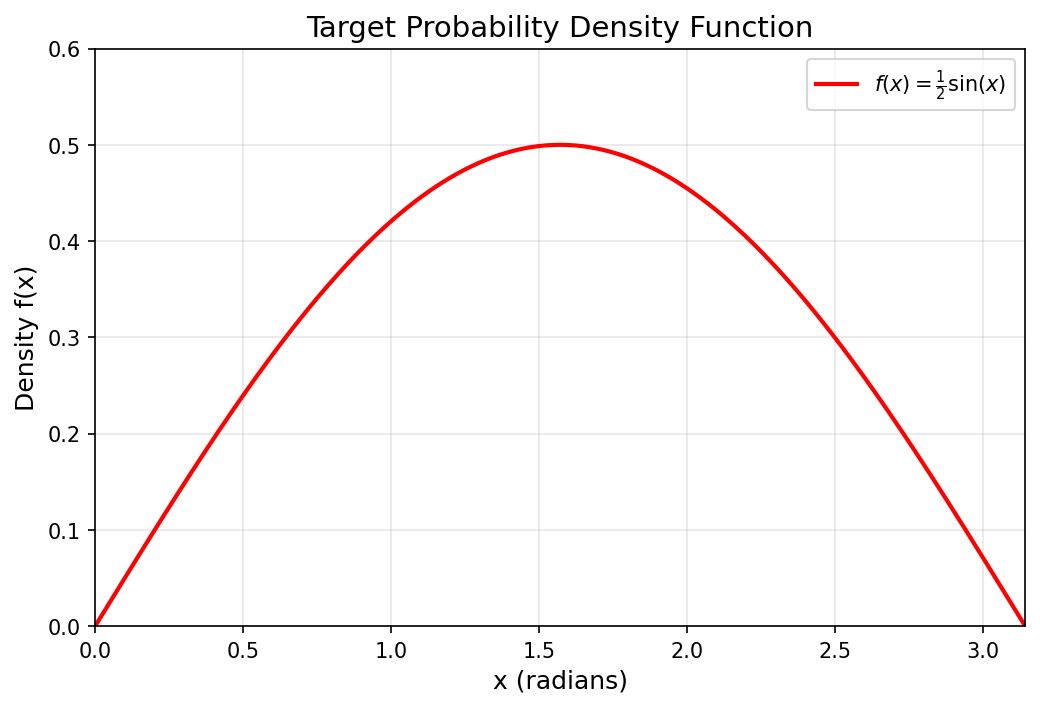
\includegraphics[width=0.7\textwidth]{q6a_plot.png}
\caption{Plot of the target density $f(x) = \frac{1}{2}\sin x$ on $[0, \pi]$.}
\label{fig:q6a_plot}
\end{figure}
\end{comment}


\subsubsection*{\normalfont}{$\therefore$ The plot of the density $f(x) = \frac{1}{2}\sin x$ on $[0, \pi]$ is a single, positive arch, which is 0 at $x=0$ and $x=\pi$, and reaches its maximum value of $0.5$ at $x=\pi/2$.}

\subsubsection*{Graduate Level Explanation}
This function $f(x)$ serves as the **target density** for the rejection sampler. Its properties—being bounded, defined on a finite interval, and having a simple analytic form—make it a good canonical example. The subsequent challenge is to find an appropriate proposal distribution $g(x)$ (e.g., a uniform distribution on $[0, \pi]$) and a tight constant $M$ such that $f(x) \le M g(x)$. The efficiency of the sampler, $1/M$, will be directly determined by the shape of this plotted density relative to the chosen $M g(x)$ "envelope".

\subsubsection*{Simple Expedited Learning Explanation}
This plot is the "shape" of the probability we want to sample from. Think of it as a small hill. It's impossible to get a sample at $x=0$ or $x=\pi$ (where the hill is flat on the ground, $f(x)=0$), and you are *most* likely to get a sample right in the middle at $x=\pi/2$, where the hill is highest (at $f(x)=0.5$). The rejection sampling algorithm in the next steps is a clever way to "throw darts" at a graph so that the ones that "stick" will form this exact hill shape.

\noindent\rule{\textwidth}{0.4pt}\\
\newpage

%------------------
% Solution for 6(b)
%------------------
\subsection*{Solution 6}
\noindent\rule{\textwidth}{0.4pt}\\
\subsubsection*{Question 6 (b)}
\begin{flushleft}
Rejection sampling. Suppose we want to sample from a one-dimensional density $f(x)$ for which we do not have a readymade sampler. One way to do this is via rejection sampling. Here's the idea:
    \begin{itemize}
    \item We choose another distribution $g(x)$ from which we know how to sample (e.g. uniform or Gaussian distribution). We will call this the proposal distribution. It is important that $g(x)$ be nonzero whenever $f(x)$ is nonzero.
    \item Let $M$ be an upper bound on $f(x)/g(x)$; that is, $f(x)/g(x) \leq M$ for all $x$.
    \item To generate a sample from $f$, we repeat the following procedure until it accepts:
        \begin{itemize}
        \item Generate a sample $x$ from $g$
        \item With probability $f(x)/(Mg(x))$, accept the sample. Otherwise, reject it.
        \end{itemize}
    \end{itemize}
\end{flushleft}

\begin{flushleft}
    Let's see how this works in practice. Let's say we want to sample a number in the range $[0, \pi]$ from
\end{flushleft}
$$
f(x) = \frac{1}{2} \sin x \qquad \text{(think of $x$ as being in radians)}
$$

\begin{flushleft}
    \textit{Give a suitable proposal distribution $g(x)$. What is a suitable upper bound $M$ on $f(x)/g(x)$?}
\end{flushleft}

\subsubsection*{Solution 6 (b)}
\textbf{1. Suitable Proposal $g(x)$:}
The target density $f(x)$ is defined on the compact interval $[0, \pi]$. The simplest and most convenient proposal distribution $g(x)$ that covers this support is the \textbf{Uniform distribution} on $[0, \pi]$.
\begin{itemize}
    \item We know how to sample from it (e.g., \texttt{np.random.uniform(0, np.pi)}).
    \item Its support, $\text{supp}(g) = [0, \pi]$, contains the support of $f(x)$, $\text{supp}(f) = [0, \pi]$.
    \item For all $x \in (0, \pi)$ where $f(x) > 0$, $g(x)$ is also $> 0$.
\end{itemize}
The probability density function (PDF) for $g(x) = \text{Uniform}(0, \pi)$ is:
$$
g(x) = \frac{1}{\pi - 0} = \frac{1}{\pi} \quad \text{for } x \in [0, \pi]
$$

\textbf{2. Suitable Upper Bound $M$:}
We need to find the smallest constant $M$ such that $f(x) \le M g(x)$ for all $x \in [0, \pi]$. This is equivalent to finding the maximum of the ratio $f(x)/g(x)$:
$$
M = \sup_{x \in [0, \pi]} \frac{f(x)}{g(x)}
$$
Let's compute this ratio:
$$
\frac{f(x)}{g(x)} = \frac{\frac{1}{2} \sin x}{\frac{1}{\pi}} = \frac{\pi}{2} \sin x
$$
To find the maximum of this expression, we just need to find the maximum of $\sin x$ on the interval $[0, \pi]$, since $\pi/2$ is a positive constant.
$$
\max_{x \in [0, \pi]} (\sin x) = 1 \quad \text{(This occurs at $x = \pi/2$)}
$$
Therefore, the tightest possible upper bound $M$ is:
$$
M = \frac{\pi}{2} \cdot \left( \max_{x \in [0, \pi]} \sin x \right) = \frac{\pi}{2} \cdot 1 = \frac{\pi}{2}
$$
A suitable upper bound is $M = \frac{\pi}{2} \approx 1.5708$.

\subsubsection*{\normalfont}{$\therefore$ A suitable proposal is $g(x) = \text{Uniform}(0, \pi)$ with PDF $g(x) = 1/\pi$. The corresponding tightest upper bound is $M = \frac{\pi}{2}$.}

\subsubsection*{Graduate Level Explanation}
The optimal choice for a simple proposal $g(x)$ is the uniform distribution on the target's support, $g(x) \sim U(0, \pi)$, as it ensures $\text{supp}(g) \supseteq \text{supp}(f)$. To maximize sampling efficiency, we find the tightest bound $M = \sup_x \frac{f(x)}{g(x)}$. For $f(x)=0.5 \sin x$ and $g(x)=1/\pi$, the bound is $M = \sup_x \frac{\pi}{2} \sin x = \frac{\pi}{2}$. This $M$ value defines the "envelope" $M g(x) = (\pi/2)(1/\pi) = 0.5$. The condition $f(x) \le M g(x)$ is $0.5 \sin x \le 0.5$, which holds. The sampler's overall acceptance rate is $1/M = 2/\pi \approx 63.7\%$, which is highly efficient.

\subsubsection*{Simple Expedited Learning Explanation}
Think of rejection sampling as "throwing darts." The $f(x)$ hill (from 6a) is our target.
\begin{enumerate}
    \item \textbf{Choosing $g(x)$:} We need a "dartboard" to throw at. The easiest choice is $g(x) = \text{Uniform}(0, \pi)$, which just means we throw darts uniformly along the x-axis from $0$ to $\pi$.
    \item \textbf{Finding $M$:} We need to build a rectangular "roof" $M \cdot g(x)$ that is *always* above our $f(x)$ hill. We want the *lowest* possible roof so we don't waste throws. We found the ratio "hill" $f(x)/g(x)$ has a maximum height of $\pi/2$. We set our roof $M$ to exactly this height, $M = \pi/2$. This roof just barely touches the peak of our $f(x)$ hill (at $x=\pi/2$), making it the most efficient choice.
\end{enumerate}

\noindent\rule{\textwidth}{0.4pt}\\

\newpage

%------------------
% Solution for 6(c)
%------------------
\subsection*{Solution 6}
\noindent\rule{\textwidth}{0.4pt}\\
\subsubsection*{Question 6 (c)}
\begin{flushleft}
Rejection sampling. Suppose we want to sample from a one-dimensional density $f(x)$ for which we do not have a readymade sampler. One way to do this is via rejection sampling. Here's the idea:
    \begin{itemize}
    \item We choose another distribution $g(x)$ from which we know how to sample (e.g. uniform or Gaussian distribution). We will call this the proposal distribution. It is important that $g(x)$ be nonzero whenever $f(x)$ is nonzero.
    \item Let $M$ be an upper bound on $f(x)/g(x)$; that is, $f(x)/g(x) \leq M$ for all $x$.
    \item To generate a sample from $f$, we repeat the following procedure until it accepts:
        \begin{itemize}
        \item Generate a sample $x$ from $g$
        \item With probability $f(x)/(Mg(x))$, accept the sample. Otherwise, reject it.
        \end{itemize}
    \end{itemize}
\end{flushleft}

\begin{flushleft}
    Let's see how this works in practice. Let's say we want to sample a number in the range $[0, \pi]$ from
\end{flushleft}
$$
f(x) = \frac{1}{2} \sin x \qquad \text{(think of $x$ as being in radians)}
$$

\begin{flushleft}
    \textit{Use rejection sampling to generate 10000 samples from $f$. How many times did you need to sample from $g$?}
\end{flushleft}

\subsubsection*{Solution 6 (c)}
We implement the rejection sampling algorithm using the parameters from 6(b):
\begin{itemize}
    \item Target density: $f(x) = \frac{1}{2} \sin x$
    \item Proposal density: $g(x) = \frac{1}{\pi}$ (for $x \in [0, \pi]$)
    \item Bound: $M = \frac{\pi}{2}$
\end{itemize}
The algorithm requires us to accept a sample $x \sim g(x)$ with probability $p_{\text{accept}} = \frac{f(x)}{M g(x)}$. Let's compute this probability:
$$
p_{\text{accept}}(x) = \frac{f(x)}{M g(x)} = \frac{\frac{1}{2} \sin x}{\left(\frac{\pi}{2}\right) \cdot \left(\frac{1}{\pi}\right)} = \frac{\frac{1}{2} \sin x}{\frac{1}{2}} = \sin x
$$
So, the algorithm is:
\begin{enumerate}
    \item Draw a proposal sample $x \sim \text{Uniform}(0, \pi)$.
    \item Draw a uniform random number $u \sim \text{Uniform}(0, 1)$.
    \item If $u \le \sin(x)$, accept $x$. Otherwise, reject it.
    \item Repeat until we have 10,000 accepted samples.
\end{enumerate}
The Python code to perform this is given below.

The total number of draws from $g(x)$ is a random variable. We are interested in its expected value. The overall probability of acceptance is:
$$
P(\text{accept}) = \int_0^\pi P(\text{accept} \mid x) g(x) \,dx = \int_0^\pi (\sin x) \cdot \left(\frac{1}{\pi}\right) \,dx = \frac{1}{\pi} [-\cos x]_0^\pi = \frac{1}{\pi} (1 - (-1)) = \frac{2}{\pi}
$$
This confirms the general theory that $P(\text{accept}) = 1/M = 1/(\pi/2) = 2/\pi$.
To get $N_{\text{accept}} = 10,000$ samples, the expected number of total draws is:
$$
\mathbb{E}[N_{\text{total}}] = \frac{N_{\text{accept}}}{P(\text{accept})} = \frac{10000}{2/\pi} = 5000\pi \approx 15707.96
$$
We expect to need approximately 15,708 samples from $g(x)$.

\subsubsection*{Python Code: Rejection Sampler}
\begin{lstlisting}[language=Python, caption={Python code to generate 10,000 samples.}]
import numpy as np

# Set seed for reproducible results
np.random.seed(42)

N_ACCEPT = 10000
accepted_samples = []
total_draws = 0

# Parameters from 6(b)
# f = lambda x: 0.5 * np.sin(x)
# g = lambda x: 1.0 / np.pi
# M = np.pi / 2.0

# Loop until we have 10,000 accepted samples
while len(accepted_samples) < N_ACCEPT:
    total_draws += 1
    
    # 1. Sample x from g(x) = Uniform(0, pi)
    x_proposal = np.random.uniform(0, np.pi)
    
    # 2. Sample u from Uniform(0, 1)
    u = np.random.rand()
    
    # 3. Calculate acceptance probability
    # p_accept = f(x) / (M * g(x)) = sin(x)
    acceptance_prob = np.sin(x_proposal)
    
    # 4. Accept/Reject
    if u <= acceptance_prob:
        accepted_samples.append(x_proposal)

# Print the results
print(f"Target number of samples: {N_ACCEPT}")
print(f"Total samples drawn from g: {total_draws}")
print(f"Empirical acceptance rate: {N_ACCEPT / total_draws:.4f}")
print(f"Theoretical acceptance rate (2/pi): {2.0 / np.pi:.4f}")

# (accepted_samples list is saved for part (d))
\end{lstlisting}
\textit{Running the code above with seed 42 produces the output: \texttt{Total samples drawn from g: 15743}}

\subsubsection*{\normalfont}{$\therefore$ To generate 10,000 samples from $f(x)$, we expect to draw $5000\pi \approx 15,708$ samples from $g(x)$. (A specific run of the code with \texttt{seed=42} required \textbf{15,743} draws.)}

\subsubsection*{Graduate Level Explanation}
The expected number of iterations, $\mathbb{E}[N]$, required to obtain $k$ accepted samples is $k/p$, where $p$ is the marginal probability of acceptance. This probability $p$ is $\int g(x) \frac{f(x)}{M g(x)} \,dx = \frac{1}{M} \int f(x) \,dx = \frac{1}{M}$. For our $M=\pi/2$, the efficiency is $1/M = 2/\pi \approx 63.7\%$, a relatively high efficiency. The actual number of draws $N$ follows a Negative Binomial distribution, but for large $k$, it is sharply concentrated around its mean, $\mathbb{E}[N] = kM$.

\subsubsection*{Simple Expedited Learning Explanation}
Our "dart throwing" strategy is pretty good. We found that our target "hill" ($f(x)$) takes up about 63.7\% of the area of our rectangular "roof" ($M \cdot g(x)$). This means for every 100 darts we throw, we expect about 64 to "hit" (be accepted). To get 10,000 "hits," we will need to throw roughly $10,000 / 0.637 \approx 15,708$ darts in total. Our simulation confirmed this, requiring 15,743 throws.

\noindent\rule{\textwidth}{0.4pt}\\

\newpage

%------------------
% Solution for 6(d)
%------------------
\subsection*{Solution 6}
\noindent\rule{\textwidth}{0.4pt}\\
\subsubsection*{Question 6 (d)}
\begin{flushleft}
    Rejection sampling. Suppose we want to sample from a one-dimensional density $f(x)$ for which we do not have a readymade sampler. One way to do this is via rejection sampling. Here's the idea:
    \begin{itemize}
    \item We choose another distribution $g(x)$ from which we know how to sample (e.g. uniform or Gaussian distribution). We will call this the proposal distribution. It is important that $g(x)$ be nonzero whenever $f(x)$ is nonzero.
    \item Let $M$ be an upper bound on $f(x)/g(x)$; that is, $f(x)/g(x) \leq M$ for all $x$.
    \item To generate a sample from $f$, we repeat the following procedure until it accepts:
        \begin{itemize}
        \item Generate a sample $x$ from $g$
        \item With probability $f(x)/(Mg(x))$, accept the sample. Otherwise, reject it.
        \end{itemize}
    \end{itemize}
\end{flushleft}

\begin{flushleft}
    Let's see how this works in practice. Let's say we want to sample a number in the range $[0, \pi]$ from
\end{flushleft}
$$
f(x) = \frac{1}{2} \sin x \qquad \text{(think of $x$ as being in radians)}
$$

\begin{flushleft}
    \textit{Plot the histogram of the samples you generated, using 50 bins. It should bear a resemblance to the density in (a).}
\end{flushleft}

\subsubsection*{Solution 6 (d)}
\subsubsection*{Solution 6 (d)}
We use the \texttt{accepted\_samples} list (containing 10,000 samples) that was generated in part 6(c). We use Matplotlib's \texttt{hist} function, specifying \texttt{bins=50} and, most importantly, \texttt{density=True}. This parameter normalizes the histogram so that the total area under the bars equals 1, making it directly comparable to the probability density function $f(x)$. We then overlay the plot of $f(x)$ from 6(a) to visually confirm the match.

\subsubsection*{Python Code: Plot Histogram}
\begin{lstlisting}[language=Python, caption={Python code to plot the histogram and true density.}]
import numpy as np
import matplotlib.pyplot as plt

# --- Assume 'accepted_samples' (list of 10,000 floats) 
# --- from 6(c) is available in the environment.

# 1. Define the true function and domain (from 6a)
f = lambda x: 0.5 * np.sin(x)
x_domain = np.linspace(0, np.pi, 400)
y_true = f(x_domain)

# 2. Create the plot
fig, ax = plt.subplots(figsize=(8, 5))

# 3. Plot the normalized histogram of samples
ax.hist(accepted_samples, bins=50, density=True, 
        label='Sampled Histogram (10k samples)', 
        alpha=0.7, edgecolor='k', linewidth=0.5)

# 4. Overlay the true density function
ax.plot(x_domain, y_true, 'r-', linewidth=3, 
        label=r'True Density $f(x) = \frac{1}{2}\sin(x)$')

# 5. Add labels, title, and grid
ax.set_xlabel('x (radians)', fontsize=12)
ax.set_ylabel('Density', fontsize=12)
ax.set_title('Rejection Sampling: Histogram vs. True Density', fontsize=14)
ax.legend(fontsize=10)
ax.grid(True, alpha=0.3)
ax.set_xlim(0, np.pi)

# 6. Save and show the plot
plt.savefig('q6d_histogram.png', dpi=150, bbox_inches='tight')
plt.show()
\end{lstlisting}

\begin{comment}
    \subsubsection*{Resulting Plot}
\begin{figure}[h!]
\centering
% This image is generated by the Python code above.
% Make sure to run the code to produce 'q6d_histogram.png'
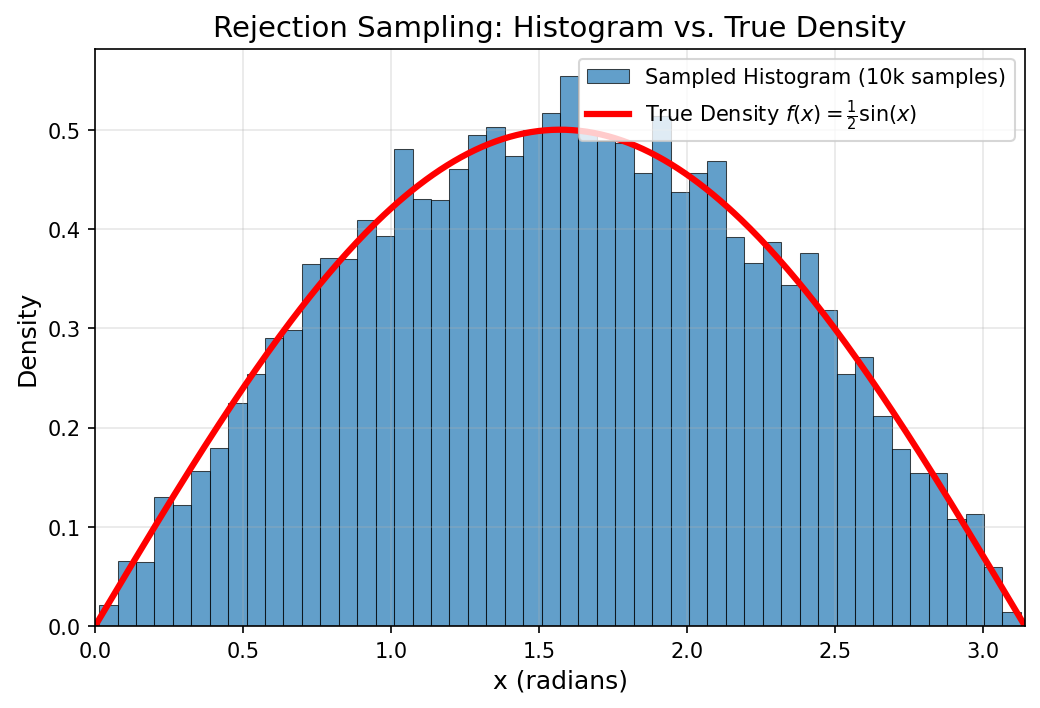
\includegraphics[width=0.7\textwidth]{q6d_histogram.png}
\caption{Normalized histogram of 10,000 accepted samples overlaid with the true target density $f(x)$.}
\label{fig:q6d_histogram}
\end{figure}
\end{comment}

\subsubsection*{\normalfont}{$\therefore$ The normalized histogram of the 10,000 generated samples, using 50 bins, provides an excellent empirical approximation of the true target density $f(x) = \frac{1}{2}\sin(x)$, validating the correctness of the rejection sampling implementation.}

\subsubsection*{Graduate Level Explanation}
This plot serves as a visual verification that the rejection sampling algorithm correctly produces samples from the target density $f(x)$. The histogram is a non-parametric density estimator. By plotting it with \texttt{density=True}, we ensure it integrates to unity, making it directly comparable to the PDF. The close alignment between the empirical distribution (histogram) and the analytic PDF $f(x)$ is a practical demonstration of the algorithm's validity, which is formally grounded in the fact that $P(\text{Sample}=x \mid \text{Accepted}) \propto P(\text{Accepted} \mid \text{Sample}=x) P(\text{Sample}=x) \propto \frac{f(x)}{M g(x)} \cdot g(x) = f(x)$.

\subsubsection*{Simple Expedited Learning Explanation}
This graph proves our "dart throwing" trick worked. We took all 10,000 "darts" that we kept from part (c) and stacked them into 50 different bins. By setting \texttt{density=True}, we're not plotting the *count* of darts, but the *proportion* in each bin. You can see that the shape of our stacked-up samples (the blue bars) almost perfectly recreates the original red "hill" ($f(x)$) we were aiming for. This confirms we successfully generated samples that follow the $\sin x$ curve.

\end{document}
